\batchmode
\documentclass[twoside]{book}

% Packages required by doxygen
\usepackage{fixltx2e}
\usepackage{calc}
\usepackage{doxygen}
\usepackage[export]{adjustbox} % also loads graphicx
\usepackage{graphicx}
\usepackage[utf8]{inputenc}
\usepackage{makeidx}
\usepackage{multicol}
\usepackage{multirow}
\PassOptionsToPackage{warn}{textcomp}
\usepackage{textcomp}
\usepackage[nointegrals]{wasysym}
\usepackage[table]{xcolor}

% Font selection
\usepackage[T1]{fontenc}
\usepackage[scaled=.90]{helvet}
\usepackage{courier}
\usepackage{amssymb}
\usepackage{sectsty}
\renewcommand{\familydefault}{\sfdefault}
\allsectionsfont{%
  \fontseries{bc}\selectfont%
  \color{darkgray}%
}
\renewcommand{\DoxyLabelFont}{%
  \fontseries{bc}\selectfont%
  \color{darkgray}%
}
\newcommand{\+}{\discretionary{\mbox{\scriptsize$\hookleftarrow$}}{}{}}

% Page & text layout
\usepackage{geometry}
\geometry{%
  a4paper,%
  top=2.5cm,%
  bottom=2.5cm,%
  left=2.5cm,%
  right=2.5cm%
}
\tolerance=750
\hfuzz=15pt
\hbadness=750
\setlength{\emergencystretch}{15pt}
\setlength{\parindent}{0cm}
\setlength{\parskip}{3ex plus 2ex minus 2ex}
\makeatletter
\renewcommand{\paragraph}{%
  \@startsection{paragraph}{4}{0ex}{-1.0ex}{1.0ex}{%
    \normalfont\normalsize\bfseries\SS@parafont%
  }%
}
\renewcommand{\subparagraph}{%
  \@startsection{subparagraph}{5}{0ex}{-1.0ex}{1.0ex}{%
    \normalfont\normalsize\bfseries\SS@subparafont%
  }%
}
\makeatother

% Headers & footers
\usepackage{fancyhdr}
\pagestyle{fancyplain}
\fancyhead[LE]{\fancyplain{}{\bfseries\thepage}}
\fancyhead[CE]{\fancyplain{}{}}
\fancyhead[RE]{\fancyplain{}{\bfseries\leftmark}}
\fancyhead[LO]{\fancyplain{}{\bfseries\rightmark}}
\fancyhead[CO]{\fancyplain{}{}}
\fancyhead[RO]{\fancyplain{}{\bfseries\thepage}}
\fancyfoot[LE]{\fancyplain{}{}}
\fancyfoot[CE]{\fancyplain{}{}}
\fancyfoot[RE]{\fancyplain{}{\bfseries\scriptsize Generated by Doxygen }}
\fancyfoot[LO]{\fancyplain{}{\bfseries\scriptsize Generated by Doxygen }}
\fancyfoot[CO]{\fancyplain{}{}}
\fancyfoot[RO]{\fancyplain{}{}}
\renewcommand{\footrulewidth}{0.4pt}
\renewcommand{\chaptermark}[1]{%
  \markboth{#1}{}%
}
\renewcommand{\sectionmark}[1]{%
  \markright{\thesection\ #1}%
}

% Indices & bibliography
\usepackage{natbib}
\usepackage[titles]{tocloft}
\setcounter{tocdepth}{3}
\setcounter{secnumdepth}{5}
\makeindex

% Hyperlinks (required, but should be loaded last)
\usepackage{ifpdf}
\ifpdf
  \usepackage[pdftex,pagebackref=true]{hyperref}
\else
  \usepackage[ps2pdf,pagebackref=true]{hyperref}
\fi
\hypersetup{%
  colorlinks=true,%
  linkcolor=blue,%
  citecolor=blue,%
  unicode%
}

% Custom commands
\newcommand{\clearemptydoublepage}{%
  \newpage{\pagestyle{empty}\cleardoublepage}%
}

\usepackage{caption}
\captionsetup{labelsep=space,justification=centering,font={bf},singlelinecheck=off,skip=4pt,position=top}

%===== C O N T E N T S =====

\begin{document}

% Titlepage & ToC
\hypersetup{pageanchor=false,
             bookmarksnumbered=true
            }
\pagenumbering{alph}
\pagenumbering{arabic}
\hypersetup{pageanchor=true}

%--- Begin generated contents ---
\chapter{Demo problem\+: Flow past a cylinder with a waving flag}
\label{index}\hypertarget{index}{}\hypertarget{index_q}{}\section{A few quick questions...}\label{index_q}
Since {\ttfamily oomph-\/lib} is developed as open-\/source software, any evidence that the code is being downloaded and used is very helpful for us as it helps to justify our continued work on this project.

We would therefore be extremely grateful if you could provide the information requested in the form below. Pressing the \char`\"{}submit\char`\"{} button will get you to the actual download page.

{\bfseries Note\+:} 
\begin{DoxyItemize}
\item All information will be treated as confidential. 
\item If you provide your email address and check the appropriate box we will add you to our mailing list to inform you of upgrades and bug fixes to the code. Rest assured that the mailing list is {\bfseries very low volume} -- we have better things to do than to bombard you with email. 
\item If you still feel reluctant to provide any of the information requested, feel free to enter some dummy input. The form will check that {\bfseries some} information has been entered but entering your name as \char`\"{}\+Joe Cool\char`\"{} is perfectly acceptable -- this is to discourage people from not providing the information simply because they are too lazy to type... 
\end{DoxyItemize}



 







 

 \hypertarget{index_pdf}{}\section{P\+D\+F file}\label{index_pdf}
A \href{../latex/refman.pdf}{\tt pdf version} of this document is available. \end{document}

\chapter{Namespace Index}
\section{Namespace List}
Here is a list of all namespaces with brief descriptions\+:\begin{DoxyCompactList}
\item\contentsline{section}{\hyperlink{namespaceGlobal__Physical__Variables}{Global\+\_\+\+Physical\+\_\+\+Variables} \\*Global variables that represent physical properties }{\pageref{namespaceGlobal__Physical__Variables}}{}
\item\contentsline{section}{\hyperlink{namespaceoomph}{oomph} }{\pageref{namespaceoomph}}{}
\item\contentsline{section}{\hyperlink{namespacePhysical__Variables}{Physical\+\_\+\+Variables} \\*Namespace for the solution of 2D linear shell equation }{\pageref{namespacePhysical__Variables}}{}
\end{DoxyCompactList}

\chapter{Hierarchical Index}
\section{Class Hierarchy}
This inheritance list is sorted roughly, but not completely, alphabetically\+:\begin{DoxyCompactList}
\item Problem\begin{DoxyCompactList}
\item \contentsline{section}{Unstructured\+Solid\+Problem$<$ E\+L\+E\+M\+E\+NT $>$}{\pageref{classUnstructuredSolidProblem}}{}
\end{DoxyCompactList}
\end{DoxyCompactList}

\chapter{Class Index}
\section{Class List}
Here are the classes, structs, unions and interfaces with brief descriptions\+:\begin{DoxyCompactList}
\item\contentsline{section}{\hyperlink{classPMLProblem}{P\+M\+L\+Problem$<$ E\+L\+E\+M\+E\+N\+T $>$} }{\pageref{classPMLProblem}}{}
\item\contentsline{section}{\hyperlink{classGlobalParameters_1_1TestPMLMapping}{Global\+Parameters\+::\+Test\+P\+M\+L\+Mapping} }{\pageref{classGlobalParameters_1_1TestPMLMapping}}{}
\end{DoxyCompactList}

\chapter{File Index}
\section{File List}
Here is a list of all files with brief descriptions\+:\begin{DoxyCompactList}
\item\contentsline{section}{\hyperlink{jeffery__orbit_8cc}{jeffery\+\_\+orbit.\+cc} }{\pageref{jeffery__orbit_8cc}}{}
\item\contentsline{section}{\hyperlink{jeffery__orbit_8txt__doxygenified_8h}{jeffery\+\_\+orbit.\+txt\+\_\+doxygenified.\+h} }{\pageref{jeffery__orbit_8txt__doxygenified_8h}}{}
\item\contentsline{section}{\hyperlink{my__taylor__hood__elements_8h}{my\+\_\+taylor\+\_\+hood\+\_\+elements.\+h} }{\pageref{my__taylor__hood__elements_8h}}{}
\end{DoxyCompactList}

\chapter{Namespace Documentation}
\hypertarget{namespaceFlag__definition}{}\section{Flag\+\_\+definition Namespace Reference}
\label{namespaceFlag__definition}\index{Flag\+\_\+definition@{Flag\+\_\+definition}}


Namespace for definition of flag boundaries.  


\subsection*{Classes}
\begin{DoxyCompactItemize}
\item 
class \hyperlink{classFlag__definition_1_1BottomOfFlag}{Bottom\+Of\+Flag}
\begin{DoxyCompactList}\small\item\em Geom\+Object that defines the lower boundary of the flag. \end{DoxyCompactList}\item 
class \hyperlink{classFlag__definition_1_1TipOfFlag}{Tip\+Of\+Flag}
\begin{DoxyCompactList}\small\item\em Geom\+Object that defines the tip of the flag. \end{DoxyCompactList}\item 
class \hyperlink{classFlag__definition_1_1TopOfFlag}{Top\+Of\+Flag}
\begin{DoxyCompactList}\small\item\em Geom\+Object that defines the upper boundary of the flag. \end{DoxyCompactList}\end{DoxyCompactItemize}
\subsection*{Functions}
\begin{DoxyCompactItemize}
\item 
Vector$<$ double $>$ \hyperlink{namespaceFlag__definition_a6af3444eee77be503be4aa8c2ef47c13}{upper\+\_\+tip} (const double \&t)
\begin{DoxyCompactList}\small\item\em Time-\/dependent vector to upper tip of the \char`\"{}flag\char`\"{}. \end{DoxyCompactList}\item 
Vector$<$ double $>$ \hyperlink{namespaceFlag__definition_a91eabcfac65c509ab3448d82db1eb988}{lower\+\_\+tip} (const double \&t)
\begin{DoxyCompactList}\small\item\em Time-\/dependent vector to bottom tip of the \char`\"{}flag\char`\"{}. \end{DoxyCompactList}\item 
void \hyperlink{namespaceFlag__definition_a61a03bffd4a34950ef9892be53c49f89}{setup} (Time $\ast$time\+\_\+pt)
\begin{DoxyCompactList}\small\item\em Create all Geom\+Objects needed to define the cylinder and the flag. \end{DoxyCompactList}\end{DoxyCompactItemize}
\subsection*{Variables}
\begin{DoxyCompactItemize}
\item 
double \hyperlink{namespaceFlag__definition_a47976a19abd58b9c31671f074ca57285}{Period} =10.\+0
\begin{DoxyCompactList}\small\item\em Period of prescribed flag oscillation. \end{DoxyCompactList}\item 
double \hyperlink{namespaceFlag__definition_a6cdf33de1fe6f94832181664d7769af7}{H} =0.\+2
\begin{DoxyCompactList}\small\item\em Height of flag. \end{DoxyCompactList}\item 
double \hyperlink{namespaceFlag__definition_a94553533bee82260731a466182369a9d}{L} =3.\+5
\begin{DoxyCompactList}\small\item\em Length of flag. \end{DoxyCompactList}\item 
double \hyperlink{namespaceFlag__definition_a60f30c718c6c67504b05dca7832be8aa}{Centre\+\_\+x} =2.\+0
\begin{DoxyCompactList}\small\item\em x position of centre of cylinder \end{DoxyCompactList}\item 
double \hyperlink{namespaceFlag__definition_a0024007edc2ad0ef647939aa6b06bde7}{Centre\+\_\+y} =2.\+0
\begin{DoxyCompactList}\small\item\em y position of centre of cylinder \end{DoxyCompactList}\item 
double \hyperlink{namespaceFlag__definition_a921d8bd82b7b267651dea625a548dfcb}{Radius} =0.\+5
\begin{DoxyCompactList}\small\item\em Radius of cylinder. \end{DoxyCompactList}\item 
double \hyperlink{namespaceFlag__definition_ad0eb269ec983b485aa24a6f2c25d2f5b}{Amplitude} =0.\+33
\begin{DoxyCompactList}\small\item\em Amplitude of tip deflection. \end{DoxyCompactList}\item 
Time $\ast$ \hyperlink{namespaceFlag__definition_adc7ca9d539ba8569c5eaa574de22c08f}{Time\+\_\+pt} =0
\begin{DoxyCompactList}\small\item\em Pointer to the global time object. \end{DoxyCompactList}\item 
\hyperlink{classFlag__definition_1_1TopOfFlag}{Top\+Of\+Flag} $\ast$ \hyperlink{namespaceFlag__definition_af602ebeb0c40d05d00961af07bf3e842}{Top\+\_\+flag\+\_\+pt} =0
\begin{DoxyCompactList}\small\item\em Pointer to Geom\+Object that bounds the upper edge of the flag. \end{DoxyCompactList}\item 
\hyperlink{classFlag__definition_1_1BottomOfFlag}{Bottom\+Of\+Flag} $\ast$ \hyperlink{namespaceFlag__definition_adde5e58da47e90ef46e1183188281f2e}{Bottom\+\_\+flag\+\_\+pt} =0
\begin{DoxyCompactList}\small\item\em Pointer to Geom\+Object that bounds the bottom edge of the flag. \end{DoxyCompactList}\item 
\hyperlink{classFlag__definition_1_1TipOfFlag}{Tip\+Of\+Flag} $\ast$ \hyperlink{namespaceFlag__definition_a17de6efd8447ee9c2bb5a1767084ecef}{Tip\+\_\+flag\+\_\+pt} =0
\begin{DoxyCompactList}\small\item\em Pointer to Geom\+Object that bounds the tip edge of the flag. \end{DoxyCompactList}\item 
Circle $\ast$ \hyperlink{namespaceFlag__definition_a87051411606f6aa4518ace9ce66a4189}{Cylinder\+\_\+pt} =0
\begin{DoxyCompactList}\small\item\em Pointer to Geom\+Object of type Circle that defines the central cylinder. \end{DoxyCompactList}\end{DoxyCompactItemize}


\subsection{Detailed Description}
Namespace for definition of flag boundaries. 

\subsection{Function Documentation}
\mbox{\Hypertarget{namespaceFlag__definition_a91eabcfac65c509ab3448d82db1eb988}\label{namespaceFlag__definition_a91eabcfac65c509ab3448d82db1eb988}} 
\index{Flag\+\_\+definition@{Flag\+\_\+definition}!lower\+\_\+tip@{lower\+\_\+tip}}
\index{lower\+\_\+tip@{lower\+\_\+tip}!Flag\+\_\+definition@{Flag\+\_\+definition}}
\subsubsection{\texorpdfstring{lower\+\_\+tip()}{lower\_tip()}}
{\footnotesize\ttfamily Vector$<$double$>$ Flag\+\_\+definition\+::lower\+\_\+tip (\begin{DoxyParamCaption}\item[{const double \&}]{t }\end{DoxyParamCaption})}



Time-\/dependent vector to bottom tip of the \char`\"{}flag\char`\"{}. 



Definition at line 112 of file turek\+\_\+flag\+\_\+non\+\_\+fsi.\+cc.



References Amplitude, and L.



Referenced by Flag\+\_\+definition\+::\+Bottom\+Of\+Flag\+::position(), and Flag\+\_\+definition\+::\+Tip\+Of\+Flag\+::position().

\mbox{\Hypertarget{namespaceFlag__definition_a61a03bffd4a34950ef9892be53c49f89}\label{namespaceFlag__definition_a61a03bffd4a34950ef9892be53c49f89}} 
\index{Flag\+\_\+definition@{Flag\+\_\+definition}!setup@{setup}}
\index{setup@{setup}!Flag\+\_\+definition@{Flag\+\_\+definition}}
\subsubsection{\texorpdfstring{setup()}{setup()}}
{\footnotesize\ttfamily void Flag\+\_\+definition\+::setup (\begin{DoxyParamCaption}\item[{Time $\ast$}]{time\+\_\+pt }\end{DoxyParamCaption})}



Create all Geom\+Objects needed to define the cylinder and the flag. 

Create Geom\+Object that bounds the upper edge of the flag

Create Geom\+Object that bounds the bottom edge of the flag

Create Geom\+Object that bounds the tip edge of the flag 

Definition at line 281 of file turek\+\_\+flag\+\_\+non\+\_\+fsi.\+cc.



Referenced by main(), and Turek\+Non\+F\+S\+I\+Problem$<$ E\+L\+E\+M\+E\+N\+T $>$\+::\+Turek\+Non\+F\+S\+I\+Problem().

\mbox{\Hypertarget{namespaceFlag__definition_a6af3444eee77be503be4aa8c2ef47c13}\label{namespaceFlag__definition_a6af3444eee77be503be4aa8c2ef47c13}} 
\index{Flag\+\_\+definition@{Flag\+\_\+definition}!upper\+\_\+tip@{upper\+\_\+tip}}
\index{upper\+\_\+tip@{upper\+\_\+tip}!Flag\+\_\+definition@{Flag\+\_\+definition}}
\subsubsection{\texorpdfstring{upper\+\_\+tip()}{upper\_tip()}}
{\footnotesize\ttfamily Vector$<$double$>$ Flag\+\_\+definition\+::upper\+\_\+tip (\begin{DoxyParamCaption}\item[{const double \&}]{t }\end{DoxyParamCaption})}



Time-\/dependent vector to upper tip of the \char`\"{}flag\char`\"{}. 



Definition at line 100 of file turek\+\_\+flag\+\_\+non\+\_\+fsi.\+cc.



References Amplitude, and L.



Referenced by Flag\+\_\+definition\+::\+Top\+Of\+Flag\+::position(), and Flag\+\_\+definition\+::\+Tip\+Of\+Flag\+::position().



\subsection{Variable Documentation}
\mbox{\Hypertarget{namespaceFlag__definition_ad0eb269ec983b485aa24a6f2c25d2f5b}\label{namespaceFlag__definition_ad0eb269ec983b485aa24a6f2c25d2f5b}} 
\index{Flag\+\_\+definition@{Flag\+\_\+definition}!Amplitude@{Amplitude}}
\index{Amplitude@{Amplitude}!Flag\+\_\+definition@{Flag\+\_\+definition}}
\subsubsection{\texorpdfstring{Amplitude}{Amplitude}}
{\footnotesize\ttfamily double Flag\+\_\+definition\+::\+Amplitude =0.\+33}



Amplitude of tip deflection. 



Definition at line 92 of file turek\+\_\+flag\+\_\+non\+\_\+fsi.\+cc.



Referenced by lower\+\_\+tip(), and upper\+\_\+tip().

\mbox{\Hypertarget{namespaceFlag__definition_adde5e58da47e90ef46e1183188281f2e}\label{namespaceFlag__definition_adde5e58da47e90ef46e1183188281f2e}} 
\index{Flag\+\_\+definition@{Flag\+\_\+definition}!Bottom\+\_\+flag\+\_\+pt@{Bottom\+\_\+flag\+\_\+pt}}
\index{Bottom\+\_\+flag\+\_\+pt@{Bottom\+\_\+flag\+\_\+pt}!Flag\+\_\+definition@{Flag\+\_\+definition}}
\subsubsection{\texorpdfstring{Bottom\+\_\+flag\+\_\+pt}{Bottom\_flag\_pt}}
{\footnotesize\ttfamily \hyperlink{classFlag__definition_1_1BottomOfFlag}{Bottom\+Of\+Flag}$\ast$ Flag\+\_\+definition\+::\+Bottom\+\_\+flag\+\_\+pt =0}



Pointer to Geom\+Object that bounds the bottom edge of the flag. 



Definition at line 271 of file turek\+\_\+flag\+\_\+non\+\_\+fsi.\+cc.



Referenced by Turek\+Non\+F\+S\+I\+Problem$<$ E\+L\+E\+M\+E\+N\+T $>$\+::\+Turek\+Non\+F\+S\+I\+Problem().

\mbox{\Hypertarget{namespaceFlag__definition_a60f30c718c6c67504b05dca7832be8aa}\label{namespaceFlag__definition_a60f30c718c6c67504b05dca7832be8aa}} 
\index{Flag\+\_\+definition@{Flag\+\_\+definition}!Centre\+\_\+x@{Centre\+\_\+x}}
\index{Centre\+\_\+x@{Centre\+\_\+x}!Flag\+\_\+definition@{Flag\+\_\+definition}}
\subsubsection{\texorpdfstring{Centre\+\_\+x}{Centre\_x}}
{\footnotesize\ttfamily double Flag\+\_\+definition\+::\+Centre\+\_\+x =2.\+0}



x position of centre of cylinder 



Definition at line 83 of file turek\+\_\+flag\+\_\+non\+\_\+fsi.\+cc.



Referenced by Turek\+Non\+F\+S\+I\+Problem$<$ E\+L\+E\+M\+E\+N\+T $>$\+::\+Turek\+Non\+F\+S\+I\+Problem().

\mbox{\Hypertarget{namespaceFlag__definition_a0024007edc2ad0ef647939aa6b06bde7}\label{namespaceFlag__definition_a0024007edc2ad0ef647939aa6b06bde7}} 
\index{Flag\+\_\+definition@{Flag\+\_\+definition}!Centre\+\_\+y@{Centre\+\_\+y}}
\index{Centre\+\_\+y@{Centre\+\_\+y}!Flag\+\_\+definition@{Flag\+\_\+definition}}
\subsubsection{\texorpdfstring{Centre\+\_\+y}{Centre\_y}}
{\footnotesize\ttfamily double Flag\+\_\+definition\+::\+Centre\+\_\+y =2.\+0}



y position of centre of cylinder 



Definition at line 86 of file turek\+\_\+flag\+\_\+non\+\_\+fsi.\+cc.



Referenced by Turek\+Non\+F\+S\+I\+Problem$<$ E\+L\+E\+M\+E\+N\+T $>$\+::\+Turek\+Non\+F\+S\+I\+Problem().

\mbox{\Hypertarget{namespaceFlag__definition_a87051411606f6aa4518ace9ce66a4189}\label{namespaceFlag__definition_a87051411606f6aa4518ace9ce66a4189}} 
\index{Flag\+\_\+definition@{Flag\+\_\+definition}!Cylinder\+\_\+pt@{Cylinder\+\_\+pt}}
\index{Cylinder\+\_\+pt@{Cylinder\+\_\+pt}!Flag\+\_\+definition@{Flag\+\_\+definition}}
\subsubsection{\texorpdfstring{Cylinder\+\_\+pt}{Cylinder\_pt}}
{\footnotesize\ttfamily Circle$\ast$ Flag\+\_\+definition\+::\+Cylinder\+\_\+pt =0}



Pointer to Geom\+Object of type Circle that defines the central cylinder. 



Definition at line 278 of file turek\+\_\+flag\+\_\+non\+\_\+fsi.\+cc.



Referenced by Turek\+Non\+F\+S\+I\+Problem$<$ E\+L\+E\+M\+E\+N\+T $>$\+::\+Turek\+Non\+F\+S\+I\+Problem().

\mbox{\Hypertarget{namespaceFlag__definition_a6cdf33de1fe6f94832181664d7769af7}\label{namespaceFlag__definition_a6cdf33de1fe6f94832181664d7769af7}} 
\index{Flag\+\_\+definition@{Flag\+\_\+definition}!H@{H}}
\index{H@{H}!Flag\+\_\+definition@{Flag\+\_\+definition}}
\subsubsection{\texorpdfstring{H}{H}}
{\footnotesize\ttfamily double Flag\+\_\+definition\+::H =0.\+2}



Height of flag. 



Definition at line 77 of file turek\+\_\+flag\+\_\+non\+\_\+fsi.\+cc.



Referenced by Turek\+Non\+F\+S\+I\+Problem$<$ E\+L\+E\+M\+E\+N\+T $>$\+::\+Turek\+Non\+F\+S\+I\+Problem().

\mbox{\Hypertarget{namespaceFlag__definition_a94553533bee82260731a466182369a9d}\label{namespaceFlag__definition_a94553533bee82260731a466182369a9d}} 
\index{Flag\+\_\+definition@{Flag\+\_\+definition}!L@{L}}
\index{L@{L}!Flag\+\_\+definition@{Flag\+\_\+definition}}
\subsubsection{\texorpdfstring{L}{L}}
{\footnotesize\ttfamily double Flag\+\_\+definition\+::L =3.\+5}



Length of flag. 



Definition at line 80 of file turek\+\_\+flag\+\_\+non\+\_\+fsi.\+cc.



Referenced by lower\+\_\+tip(), Turek\+Non\+F\+S\+I\+Problem$<$ E\+L\+E\+M\+E\+N\+T $>$\+::\+Turek\+Non\+F\+S\+I\+Problem(), and upper\+\_\+tip().

\mbox{\Hypertarget{namespaceFlag__definition_a47976a19abd58b9c31671f074ca57285}\label{namespaceFlag__definition_a47976a19abd58b9c31671f074ca57285}} 
\index{Flag\+\_\+definition@{Flag\+\_\+definition}!Period@{Period}}
\index{Period@{Period}!Flag\+\_\+definition@{Flag\+\_\+definition}}
\subsubsection{\texorpdfstring{Period}{Period}}
{\footnotesize\ttfamily double Flag\+\_\+definition\+::\+Period =10.\+0}



Period of prescribed flag oscillation. 



Definition at line 74 of file turek\+\_\+flag\+\_\+non\+\_\+fsi.\+cc.



Referenced by main(), Flag\+\_\+definition\+::\+Top\+Of\+Flag\+::position(), and Flag\+\_\+definition\+::\+Bottom\+Of\+Flag\+::position().

\mbox{\Hypertarget{namespaceFlag__definition_a921d8bd82b7b267651dea625a548dfcb}\label{namespaceFlag__definition_a921d8bd82b7b267651dea625a548dfcb}} 
\index{Flag\+\_\+definition@{Flag\+\_\+definition}!Radius@{Radius}}
\index{Radius@{Radius}!Flag\+\_\+definition@{Flag\+\_\+definition}}
\subsubsection{\texorpdfstring{Radius}{Radius}}
{\footnotesize\ttfamily double Flag\+\_\+definition\+::\+Radius =0.\+5}



Radius of cylinder. 



Definition at line 89 of file turek\+\_\+flag\+\_\+non\+\_\+fsi.\+cc.



Referenced by Turek\+Non\+F\+S\+I\+Problem$<$ E\+L\+E\+M\+E\+N\+T $>$\+::\+Turek\+Non\+F\+S\+I\+Problem().

\mbox{\Hypertarget{namespaceFlag__definition_adc7ca9d539ba8569c5eaa574de22c08f}\label{namespaceFlag__definition_adc7ca9d539ba8569c5eaa574de22c08f}} 
\index{Flag\+\_\+definition@{Flag\+\_\+definition}!Time\+\_\+pt@{Time\+\_\+pt}}
\index{Time\+\_\+pt@{Time\+\_\+pt}!Flag\+\_\+definition@{Flag\+\_\+definition}}
\subsubsection{\texorpdfstring{Time\+\_\+pt}{Time\_pt}}
{\footnotesize\ttfamily Time$\ast$ Flag\+\_\+definition\+::\+Time\+\_\+pt =0}



Pointer to the global time object. 



Definition at line 95 of file turek\+\_\+flag\+\_\+non\+\_\+fsi.\+cc.

\mbox{\Hypertarget{namespaceFlag__definition_a17de6efd8447ee9c2bb5a1767084ecef}\label{namespaceFlag__definition_a17de6efd8447ee9c2bb5a1767084ecef}} 
\index{Flag\+\_\+definition@{Flag\+\_\+definition}!Tip\+\_\+flag\+\_\+pt@{Tip\+\_\+flag\+\_\+pt}}
\index{Tip\+\_\+flag\+\_\+pt@{Tip\+\_\+flag\+\_\+pt}!Flag\+\_\+definition@{Flag\+\_\+definition}}
\subsubsection{\texorpdfstring{Tip\+\_\+flag\+\_\+pt}{Tip\_flag\_pt}}
{\footnotesize\ttfamily \hyperlink{classFlag__definition_1_1TipOfFlag}{Tip\+Of\+Flag}$\ast$ Flag\+\_\+definition\+::\+Tip\+\_\+flag\+\_\+pt =0}



Pointer to Geom\+Object that bounds the tip edge of the flag. 



Definition at line 274 of file turek\+\_\+flag\+\_\+non\+\_\+fsi.\+cc.



Referenced by Turek\+Non\+F\+S\+I\+Problem$<$ E\+L\+E\+M\+E\+N\+T $>$\+::\+Turek\+Non\+F\+S\+I\+Problem().

\mbox{\Hypertarget{namespaceFlag__definition_af602ebeb0c40d05d00961af07bf3e842}\label{namespaceFlag__definition_af602ebeb0c40d05d00961af07bf3e842}} 
\index{Flag\+\_\+definition@{Flag\+\_\+definition}!Top\+\_\+flag\+\_\+pt@{Top\+\_\+flag\+\_\+pt}}
\index{Top\+\_\+flag\+\_\+pt@{Top\+\_\+flag\+\_\+pt}!Flag\+\_\+definition@{Flag\+\_\+definition}}
\subsubsection{\texorpdfstring{Top\+\_\+flag\+\_\+pt}{Top\_flag\_pt}}
{\footnotesize\ttfamily \hyperlink{classFlag__definition_1_1TopOfFlag}{Top\+Of\+Flag}$\ast$ Flag\+\_\+definition\+::\+Top\+\_\+flag\+\_\+pt =0}



Pointer to Geom\+Object that bounds the upper edge of the flag. 



Definition at line 268 of file turek\+\_\+flag\+\_\+non\+\_\+fsi.\+cc.



Referenced by Turek\+Non\+F\+S\+I\+Problem$<$ E\+L\+E\+M\+E\+N\+T $>$\+::\+Turek\+Non\+F\+S\+I\+Problem().


\hypertarget{namespaceGlobal__Parameters}{}\section{Global\+\_\+\+Parameters Namespace Reference}
\label{namespaceGlobal__Parameters}\index{Global\+\_\+\+Parameters@{Global\+\_\+\+Parameters}}


Global variables.  


\subsection*{Functions}
\begin{DoxyCompactItemize}
\item 
void \hyperlink{namespaceGlobal__Parameters_a200109847bf4cc26da4d00e8d68d569e}{gravity} (const double \&time, const Vector$<$ double $>$ \&xi, Vector$<$ double $>$ \&b)
\begin{DoxyCompactList}\small\item\em Non-\/dimensional gravity as body force. \end{DoxyCompactList}\item 
double \hyperlink{namespaceGlobal__Parameters_a536aa5314a6cdb36af852e9513351d55}{flux} (const double \&t)
\begin{DoxyCompactList}\small\item\em Flux increases between Min\+\_\+flux and Max\+\_\+flux over period Ramp\+\_\+period. \end{DoxyCompactList}\item 
void \hyperlink{namespaceGlobal__Parameters_a8c333f9041cad78d5c0160a8e2c169f5}{set\+\_\+parameters} (const string \&case\+\_\+id)
\begin{DoxyCompactList}\small\item\em Set parameters for the various test cases. \end{DoxyCompactList}\end{DoxyCompactItemize}
\subsection*{Variables}
\begin{DoxyCompactItemize}
\item 
string \hyperlink{namespaceGlobal__Parameters_a887474a9be53363806b4de417f660dba}{Case\+\_\+\+ID} =\char`\"{}F\+S\+I1\char`\"{}
\begin{DoxyCompactList}\small\item\em Default case ID. \end{DoxyCompactList}\item 
double \hyperlink{namespaceGlobal__Parameters_a9d72e94a9305c6a310940a6a427ebe06}{Re} =20.\+0
\begin{DoxyCompactList}\small\item\em Reynolds number (default assignment for F\+S\+I1 test case) \end{DoxyCompactList}\item 
double \hyperlink{namespaceGlobal__Parameters_af1af40a0df651e86bc1be273fafa98da}{St} =0.\+5
\begin{DoxyCompactList}\small\item\em Strouhal number (default assignment for F\+S\+I1 test case) \end{DoxyCompactList}\item 
double \hyperlink{namespaceGlobal__Parameters_a7a59a32365e87566069e458dc83bd18a}{Re\+St} =10.\+0
\begin{DoxyCompactList}\small\item\em Product of Reynolds and Strouhal numbers (default assignment for F\+S\+I1 test case) \end{DoxyCompactList}\item 
double \hyperlink{namespaceGlobal__Parameters_a7814fddf663e56168174a42d2cd6b4c1}{Q} =1.\+429e-\/6
\begin{DoxyCompactList}\small\item\em F\+SI parameter (default assignment for F\+S\+I1 test case) \end{DoxyCompactList}\item 
double \hyperlink{namespaceGlobal__Parameters_a517d4c31b8bce6563c2f605266dd9679}{Density\+\_\+ratio} =1.\+0
\begin{DoxyCompactList}\small\item\em Density ratio (solid to fluid; default assignment for F\+S\+I1 test case) \end{DoxyCompactList}\item 
double \hyperlink{namespaceGlobal__Parameters_ab360628e7830e43e355ce5768f6d6a6c}{H} =0.\+2
\begin{DoxyCompactList}\small\item\em Height of flag. \end{DoxyCompactList}\item 
double \hyperlink{namespaceGlobal__Parameters_a0f0247cc83ba202413b50e7b4b7fceb0}{Centre\+\_\+x} =2.\+0
\begin{DoxyCompactList}\small\item\em x position of centre of cylinder \end{DoxyCompactList}\item 
double \hyperlink{namespaceGlobal__Parameters_af41282d812fdff4867e3d8c825886290}{Centre\+\_\+y} =2.\+0
\begin{DoxyCompactList}\small\item\em y position of centre of cylinder \end{DoxyCompactList}\item 
double \hyperlink{namespaceGlobal__Parameters_a126c1e491ef187867b6b7bfb52b476ad}{Radius} =0.\+5
\begin{DoxyCompactList}\small\item\em Radius of cylinder. \end{DoxyCompactList}\item 
Constitutive\+Law $\ast$ \hyperlink{namespaceGlobal__Parameters_adbd1f040f375c96fe56b3f475f7dbec2}{Constitutive\+\_\+law\+\_\+pt} =0
\begin{DoxyCompactList}\small\item\em Pointer to constitutive law. \end{DoxyCompactList}\item 
double \hyperlink{namespaceGlobal__Parameters_a3e3428638f89f970fcf2148b0bab1465}{Lambda\+\_\+sq} =0.\+0
\begin{DoxyCompactList}\small\item\em Timescale ratio for solid (dependent parameter assigned in \hyperlink{namespaceGlobal__Parameters_a8c333f9041cad78d5c0160a8e2c169f5}{set\+\_\+parameters()}) \end{DoxyCompactList}\item 
double \hyperlink{namespaceGlobal__Parameters_ab29c9f716872de235c78e62bce2c4109}{Dt} =0.\+1
\begin{DoxyCompactList}\small\item\em Timestep. \end{DoxyCompactList}\item 
bool \hyperlink{namespaceGlobal__Parameters_aac13d615d2acd78d22a3137ffd62f7aa}{Ignore\+\_\+fluid\+\_\+loading} =false
\begin{DoxyCompactList}\small\item\em Ignore fluid (default assignment for F\+S\+I1 test case) \end{DoxyCompactList}\item 
double \hyperlink{namespaceGlobal__Parameters_aa3dfbdb1b2fd80d516850f66c96b6fd0}{E} =1.\+0
\begin{DoxyCompactList}\small\item\em Elastic modulus. \end{DoxyCompactList}\item 
double \hyperlink{namespaceGlobal__Parameters_a20fccdcfa2c15ad8b951b9ada3bb1661}{Nu} =0.\+4
\begin{DoxyCompactList}\small\item\em Poisson\textquotesingle{}s ratio. \end{DoxyCompactList}\item 
double \hyperlink{namespaceGlobal__Parameters_a335000b5db4206486a116ae0468d2d0c}{Gravity} =0.\+0
\begin{DoxyCompactList}\small\item\em Non-\/dim gravity (default assignment for F\+S\+I1 test case) \end{DoxyCompactList}\item 
double \hyperlink{namespaceGlobal__Parameters_af6afcca0b1ffdf88144f99cdfed18d3b}{Ramp\+\_\+period} =2.\+0
\begin{DoxyCompactList}\small\item\em Period for ramping up in flux. \end{DoxyCompactList}\item 
double \hyperlink{namespaceGlobal__Parameters_a5aabde2d31d07e5d0a84f6ff02c263dc}{Min\+\_\+flux} =0.\+0
\begin{DoxyCompactList}\small\item\em Min. flux. \end{DoxyCompactList}\item 
double \hyperlink{namespaceGlobal__Parameters_a13f0d5d16393d21bbc904aea5cff4ea4}{Max\+\_\+flux} =1.\+0
\begin{DoxyCompactList}\small\item\em Max. flux. \end{DoxyCompactList}\end{DoxyCompactItemize}


\subsection{Detailed Description}
Global variables. 

\subsection{Function Documentation}
\mbox{\Hypertarget{namespaceGlobal__Parameters_a536aa5314a6cdb36af852e9513351d55}\label{namespaceGlobal__Parameters_a536aa5314a6cdb36af852e9513351d55}} 
\index{Global\+\_\+\+Parameters@{Global\+\_\+\+Parameters}!flux@{flux}}
\index{flux@{flux}!Global\+\_\+\+Parameters@{Global\+\_\+\+Parameters}}
\subsubsection{\texorpdfstring{flux()}{flux()}}
{\footnotesize\ttfamily double Global\+\_\+\+Parameters\+::flux (\begin{DoxyParamCaption}\item[{const double \&}]{t }\end{DoxyParamCaption})}



Flux increases between Min\+\_\+flux and Max\+\_\+flux over period Ramp\+\_\+period. 



Definition at line 132 of file turek\+\_\+flag.\+cc.



References Max\+\_\+flux, and Min\+\_\+flux.



Referenced by Turek\+Problem$<$ F\+L\+U\+I\+D\+\_\+\+E\+L\+E\+M\+E\+N\+T, S\+O\+L\+I\+D\+\_\+\+E\+L\+E\+M\+E\+N\+T $>$\+::actions\+\_\+before\+\_\+implicit\+\_\+timestep(), Turek\+Problem$<$ F\+L\+U\+I\+D\+\_\+\+E\+L\+E\+M\+E\+N\+T, S\+O\+L\+I\+D\+\_\+\+E\+L\+E\+M\+E\+N\+T $>$\+::doc\+\_\+solution(), and Turek\+Problem$<$ F\+L\+U\+I\+D\+\_\+\+E\+L\+E\+M\+E\+N\+T, S\+O\+L\+I\+D\+\_\+\+E\+L\+E\+M\+E\+N\+T $>$\+::\+Turek\+Problem().

\mbox{\Hypertarget{namespaceGlobal__Parameters_a200109847bf4cc26da4d00e8d68d569e}\label{namespaceGlobal__Parameters_a200109847bf4cc26da4d00e8d68d569e}} 
\index{Global\+\_\+\+Parameters@{Global\+\_\+\+Parameters}!gravity@{gravity}}
\index{gravity@{gravity}!Global\+\_\+\+Parameters@{Global\+\_\+\+Parameters}}
\subsubsection{\texorpdfstring{gravity()}{gravity()}}
{\footnotesize\ttfamily void Global\+\_\+\+Parameters\+::gravity (\begin{DoxyParamCaption}\item[{const double \&}]{time,  }\item[{const Vector$<$ double $>$ \&}]{xi,  }\item[{Vector$<$ double $>$ \&}]{b }\end{DoxyParamCaption})}



Non-\/dimensional gravity as body force. 



Definition at line 113 of file turek\+\_\+flag.\+cc.



References Gravity.



Referenced by Turek\+Problem$<$ F\+L\+U\+I\+D\+\_\+\+E\+L\+E\+M\+E\+N\+T, S\+O\+L\+I\+D\+\_\+\+E\+L\+E\+M\+E\+N\+T $>$\+::\+Turek\+Problem().

\mbox{\Hypertarget{namespaceGlobal__Parameters_a8c333f9041cad78d5c0160a8e2c169f5}\label{namespaceGlobal__Parameters_a8c333f9041cad78d5c0160a8e2c169f5}} 
\index{Global\+\_\+\+Parameters@{Global\+\_\+\+Parameters}!set\+\_\+parameters@{set\+\_\+parameters}}
\index{set\+\_\+parameters@{set\+\_\+parameters}!Global\+\_\+\+Parameters@{Global\+\_\+\+Parameters}}
\subsubsection{\texorpdfstring{set\+\_\+parameters()}{set\_parameters()}}
{\footnotesize\ttfamily void Global\+\_\+\+Parameters\+::set\+\_\+parameters (\begin{DoxyParamCaption}\item[{const string \&}]{case\+\_\+id }\end{DoxyParamCaption})}



Set parameters for the various test cases. 



Definition at line 147 of file turek\+\_\+flag.\+cc.



References St.



Referenced by main().



\subsection{Variable Documentation}
\mbox{\Hypertarget{namespaceGlobal__Parameters_a887474a9be53363806b4de417f660dba}\label{namespaceGlobal__Parameters_a887474a9be53363806b4de417f660dba}} 
\index{Global\+\_\+\+Parameters@{Global\+\_\+\+Parameters}!Case\+\_\+\+ID@{Case\+\_\+\+ID}}
\index{Case\+\_\+\+ID@{Case\+\_\+\+ID}!Global\+\_\+\+Parameters@{Global\+\_\+\+Parameters}}
\subsubsection{\texorpdfstring{Case\+\_\+\+ID}{Case\_ID}}
{\footnotesize\ttfamily string Global\+\_\+\+Parameters\+::\+Case\+\_\+\+ID =\char`\"{}F\+S\+I1\char`\"{}}



Default case ID. 



Definition at line 59 of file turek\+\_\+flag.\+cc.



Referenced by main().

\mbox{\Hypertarget{namespaceGlobal__Parameters_a0f0247cc83ba202413b50e7b4b7fceb0}\label{namespaceGlobal__Parameters_a0f0247cc83ba202413b50e7b4b7fceb0}} 
\index{Global\+\_\+\+Parameters@{Global\+\_\+\+Parameters}!Centre\+\_\+x@{Centre\+\_\+x}}
\index{Centre\+\_\+x@{Centre\+\_\+x}!Global\+\_\+\+Parameters@{Global\+\_\+\+Parameters}}
\subsubsection{\texorpdfstring{Centre\+\_\+x}{Centre\_x}}
{\footnotesize\ttfamily double Global\+\_\+\+Parameters\+::\+Centre\+\_\+x =2.\+0}



x position of centre of cylinder 



Definition at line 82 of file turek\+\_\+flag.\+cc.



Referenced by Turek\+Problem$<$ F\+L\+U\+I\+D\+\_\+\+E\+L\+E\+M\+E\+N\+T, S\+O\+L\+I\+D\+\_\+\+E\+L\+E\+M\+E\+N\+T $>$\+::\+Turek\+Problem().

\mbox{\Hypertarget{namespaceGlobal__Parameters_af41282d812fdff4867e3d8c825886290}\label{namespaceGlobal__Parameters_af41282d812fdff4867e3d8c825886290}} 
\index{Global\+\_\+\+Parameters@{Global\+\_\+\+Parameters}!Centre\+\_\+y@{Centre\+\_\+y}}
\index{Centre\+\_\+y@{Centre\+\_\+y}!Global\+\_\+\+Parameters@{Global\+\_\+\+Parameters}}
\subsubsection{\texorpdfstring{Centre\+\_\+y}{Centre\_y}}
{\footnotesize\ttfamily double Global\+\_\+\+Parameters\+::\+Centre\+\_\+y =2.\+0}



y position of centre of cylinder 



Definition at line 85 of file turek\+\_\+flag.\+cc.



Referenced by Turek\+Problem$<$ F\+L\+U\+I\+D\+\_\+\+E\+L\+E\+M\+E\+N\+T, S\+O\+L\+I\+D\+\_\+\+E\+L\+E\+M\+E\+N\+T $>$\+::\+Turek\+Problem().

\mbox{\Hypertarget{namespaceGlobal__Parameters_adbd1f040f375c96fe56b3f475f7dbec2}\label{namespaceGlobal__Parameters_adbd1f040f375c96fe56b3f475f7dbec2}} 
\index{Global\+\_\+\+Parameters@{Global\+\_\+\+Parameters}!Constitutive\+\_\+law\+\_\+pt@{Constitutive\+\_\+law\+\_\+pt}}
\index{Constitutive\+\_\+law\+\_\+pt@{Constitutive\+\_\+law\+\_\+pt}!Global\+\_\+\+Parameters@{Global\+\_\+\+Parameters}}
\subsubsection{\texorpdfstring{Constitutive\+\_\+law\+\_\+pt}{Constitutive\_law\_pt}}
{\footnotesize\ttfamily Constitutive\+Law$\ast$ Global\+\_\+\+Parameters\+::\+Constitutive\+\_\+law\+\_\+pt =0}



Pointer to constitutive law. 



Definition at line 91 of file turek\+\_\+flag.\+cc.



Referenced by Turek\+Problem$<$ F\+L\+U\+I\+D\+\_\+\+E\+L\+E\+M\+E\+N\+T, S\+O\+L\+I\+D\+\_\+\+E\+L\+E\+M\+E\+N\+T $>$\+::\+Turek\+Problem().

\mbox{\Hypertarget{namespaceGlobal__Parameters_a517d4c31b8bce6563c2f605266dd9679}\label{namespaceGlobal__Parameters_a517d4c31b8bce6563c2f605266dd9679}} 
\index{Global\+\_\+\+Parameters@{Global\+\_\+\+Parameters}!Density\+\_\+ratio@{Density\+\_\+ratio}}
\index{Density\+\_\+ratio@{Density\+\_\+ratio}!Global\+\_\+\+Parameters@{Global\+\_\+\+Parameters}}
\subsubsection{\texorpdfstring{Density\+\_\+ratio}{Density\_ratio}}
{\footnotesize\ttfamily double Global\+\_\+\+Parameters\+::\+Density\+\_\+ratio =1.\+0}



Density ratio (solid to fluid; default assignment for F\+S\+I1 test case) 



Definition at line 76 of file turek\+\_\+flag.\+cc.

\mbox{\Hypertarget{namespaceGlobal__Parameters_ab29c9f716872de235c78e62bce2c4109}\label{namespaceGlobal__Parameters_ab29c9f716872de235c78e62bce2c4109}} 
\index{Global\+\_\+\+Parameters@{Global\+\_\+\+Parameters}!Dt@{Dt}}
\index{Dt@{Dt}!Global\+\_\+\+Parameters@{Global\+\_\+\+Parameters}}
\subsubsection{\texorpdfstring{Dt}{Dt}}
{\footnotesize\ttfamily double Global\+\_\+\+Parameters\+::\+Dt =0.\+1}



Timestep. 



Definition at line 98 of file turek\+\_\+flag.\+cc.



Referenced by main().

\mbox{\Hypertarget{namespaceGlobal__Parameters_aa3dfbdb1b2fd80d516850f66c96b6fd0}\label{namespaceGlobal__Parameters_aa3dfbdb1b2fd80d516850f66c96b6fd0}} 
\index{Global\+\_\+\+Parameters@{Global\+\_\+\+Parameters}!E@{E}}
\index{E@{E}!Global\+\_\+\+Parameters@{Global\+\_\+\+Parameters}}
\subsubsection{\texorpdfstring{E}{E}}
{\footnotesize\ttfamily double Global\+\_\+\+Parameters\+::E =1.\+0}



Elastic modulus. 



Definition at line 104 of file turek\+\_\+flag.\+cc.

\mbox{\Hypertarget{namespaceGlobal__Parameters_a335000b5db4206486a116ae0468d2d0c}\label{namespaceGlobal__Parameters_a335000b5db4206486a116ae0468d2d0c}} 
\index{Global\+\_\+\+Parameters@{Global\+\_\+\+Parameters}!Gravity@{Gravity}}
\index{Gravity@{Gravity}!Global\+\_\+\+Parameters@{Global\+\_\+\+Parameters}}
\subsubsection{\texorpdfstring{Gravity}{Gravity}}
{\footnotesize\ttfamily double Global\+\_\+\+Parameters\+::\+Gravity =0.\+0}



Non-\/dim gravity (default assignment for F\+S\+I1 test case) 



Definition at line 110 of file turek\+\_\+flag.\+cc.



Referenced by gravity().

\mbox{\Hypertarget{namespaceGlobal__Parameters_ab360628e7830e43e355ce5768f6d6a6c}\label{namespaceGlobal__Parameters_ab360628e7830e43e355ce5768f6d6a6c}} 
\index{Global\+\_\+\+Parameters@{Global\+\_\+\+Parameters}!H@{H}}
\index{H@{H}!Global\+\_\+\+Parameters@{Global\+\_\+\+Parameters}}
\subsubsection{\texorpdfstring{H}{H}}
{\footnotesize\ttfamily double Global\+\_\+\+Parameters\+::H =0.\+2}



Height of flag. 



Definition at line 79 of file turek\+\_\+flag.\+cc.



Referenced by Turek\+Problem$<$ F\+L\+U\+I\+D\+\_\+\+E\+L\+E\+M\+E\+N\+T, S\+O\+L\+I\+D\+\_\+\+E\+L\+E\+M\+E\+N\+T $>$\+::\+Turek\+Problem().

\mbox{\Hypertarget{namespaceGlobal__Parameters_aac13d615d2acd78d22a3137ffd62f7aa}\label{namespaceGlobal__Parameters_aac13d615d2acd78d22a3137ffd62f7aa}} 
\index{Global\+\_\+\+Parameters@{Global\+\_\+\+Parameters}!Ignore\+\_\+fluid\+\_\+loading@{Ignore\+\_\+fluid\+\_\+loading}}
\index{Ignore\+\_\+fluid\+\_\+loading@{Ignore\+\_\+fluid\+\_\+loading}!Global\+\_\+\+Parameters@{Global\+\_\+\+Parameters}}
\subsubsection{\texorpdfstring{Ignore\+\_\+fluid\+\_\+loading}{Ignore\_fluid\_loading}}
{\footnotesize\ttfamily bool Global\+\_\+\+Parameters\+::\+Ignore\+\_\+fluid\+\_\+loading =false}



Ignore fluid (default assignment for F\+S\+I1 test case) 



Definition at line 101 of file turek\+\_\+flag.\+cc.



Referenced by Turek\+Problem$<$ F\+L\+U\+I\+D\+\_\+\+E\+L\+E\+M\+E\+N\+T, S\+O\+L\+I\+D\+\_\+\+E\+L\+E\+M\+E\+N\+T $>$\+::actions\+\_\+after\+\_\+adapt(), and Turek\+Problem$<$ F\+L\+U\+I\+D\+\_\+\+E\+L\+E\+M\+E\+N\+T, S\+O\+L\+I\+D\+\_\+\+E\+L\+E\+M\+E\+N\+T $>$\+::\+Turek\+Problem().

\mbox{\Hypertarget{namespaceGlobal__Parameters_a3e3428638f89f970fcf2148b0bab1465}\label{namespaceGlobal__Parameters_a3e3428638f89f970fcf2148b0bab1465}} 
\index{Global\+\_\+\+Parameters@{Global\+\_\+\+Parameters}!Lambda\+\_\+sq@{Lambda\+\_\+sq}}
\index{Lambda\+\_\+sq@{Lambda\+\_\+sq}!Global\+\_\+\+Parameters@{Global\+\_\+\+Parameters}}
\subsubsection{\texorpdfstring{Lambda\+\_\+sq}{Lambda\_sq}}
{\footnotesize\ttfamily double Global\+\_\+\+Parameters\+::\+Lambda\+\_\+sq =0.\+0}



Timescale ratio for solid (dependent parameter assigned in \hyperlink{namespaceGlobal__Parameters_a8c333f9041cad78d5c0160a8e2c169f5}{set\+\_\+parameters()}) 



Definition at line 95 of file turek\+\_\+flag.\+cc.



Referenced by Turek\+Problem$<$ F\+L\+U\+I\+D\+\_\+\+E\+L\+E\+M\+E\+N\+T, S\+O\+L\+I\+D\+\_\+\+E\+L\+E\+M\+E\+N\+T $>$\+::\+Turek\+Problem().

\mbox{\Hypertarget{namespaceGlobal__Parameters_a13f0d5d16393d21bbc904aea5cff4ea4}\label{namespaceGlobal__Parameters_a13f0d5d16393d21bbc904aea5cff4ea4}} 
\index{Global\+\_\+\+Parameters@{Global\+\_\+\+Parameters}!Max\+\_\+flux@{Max\+\_\+flux}}
\index{Max\+\_\+flux@{Max\+\_\+flux}!Global\+\_\+\+Parameters@{Global\+\_\+\+Parameters}}
\subsubsection{\texorpdfstring{Max\+\_\+flux}{Max\_flux}}
{\footnotesize\ttfamily double Global\+\_\+\+Parameters\+::\+Max\+\_\+flux =1.\+0}



Max. flux. 



Definition at line 128 of file turek\+\_\+flag.\+cc.



Referenced by flux().

\mbox{\Hypertarget{namespaceGlobal__Parameters_a5aabde2d31d07e5d0a84f6ff02c263dc}\label{namespaceGlobal__Parameters_a5aabde2d31d07e5d0a84f6ff02c263dc}} 
\index{Global\+\_\+\+Parameters@{Global\+\_\+\+Parameters}!Min\+\_\+flux@{Min\+\_\+flux}}
\index{Min\+\_\+flux@{Min\+\_\+flux}!Global\+\_\+\+Parameters@{Global\+\_\+\+Parameters}}
\subsubsection{\texorpdfstring{Min\+\_\+flux}{Min\_flux}}
{\footnotesize\ttfamily double Global\+\_\+\+Parameters\+::\+Min\+\_\+flux =0.\+0}



Min. flux. 



Definition at line 125 of file turek\+\_\+flag.\+cc.



Referenced by flux().

\mbox{\Hypertarget{namespaceGlobal__Parameters_a20fccdcfa2c15ad8b951b9ada3bb1661}\label{namespaceGlobal__Parameters_a20fccdcfa2c15ad8b951b9ada3bb1661}} 
\index{Global\+\_\+\+Parameters@{Global\+\_\+\+Parameters}!Nu@{Nu}}
\index{Nu@{Nu}!Global\+\_\+\+Parameters@{Global\+\_\+\+Parameters}}
\subsubsection{\texorpdfstring{Nu}{Nu}}
{\footnotesize\ttfamily double Global\+\_\+\+Parameters\+::\+Nu =0.\+4}



Poisson\textquotesingle{}s ratio. 



Definition at line 107 of file turek\+\_\+flag.\+cc.

\mbox{\Hypertarget{namespaceGlobal__Parameters_a7814fddf663e56168174a42d2cd6b4c1}\label{namespaceGlobal__Parameters_a7814fddf663e56168174a42d2cd6b4c1}} 
\index{Global\+\_\+\+Parameters@{Global\+\_\+\+Parameters}!Q@{Q}}
\index{Q@{Q}!Global\+\_\+\+Parameters@{Global\+\_\+\+Parameters}}
\subsubsection{\texorpdfstring{Q}{Q}}
{\footnotesize\ttfamily double Global\+\_\+\+Parameters\+::Q =1.\+429e-\/6}



F\+SI parameter (default assignment for F\+S\+I1 test case) 



Definition at line 72 of file turek\+\_\+flag.\+cc.



Referenced by Turek\+Problem$<$ F\+L\+U\+I\+D\+\_\+\+E\+L\+E\+M\+E\+N\+T, S\+O\+L\+I\+D\+\_\+\+E\+L\+E\+M\+E\+N\+T $>$\+::\+Turek\+Problem().

\mbox{\Hypertarget{namespaceGlobal__Parameters_a126c1e491ef187867b6b7bfb52b476ad}\label{namespaceGlobal__Parameters_a126c1e491ef187867b6b7bfb52b476ad}} 
\index{Global\+\_\+\+Parameters@{Global\+\_\+\+Parameters}!Radius@{Radius}}
\index{Radius@{Radius}!Global\+\_\+\+Parameters@{Global\+\_\+\+Parameters}}
\subsubsection{\texorpdfstring{Radius}{Radius}}
{\footnotesize\ttfamily double Global\+\_\+\+Parameters\+::\+Radius =0.\+5}



Radius of cylinder. 



Definition at line 88 of file turek\+\_\+flag.\+cc.



Referenced by Turek\+Problem$<$ F\+L\+U\+I\+D\+\_\+\+E\+L\+E\+M\+E\+N\+T, S\+O\+L\+I\+D\+\_\+\+E\+L\+E\+M\+E\+N\+T $>$\+::\+Turek\+Problem().

\mbox{\Hypertarget{namespaceGlobal__Parameters_af6afcca0b1ffdf88144f99cdfed18d3b}\label{namespaceGlobal__Parameters_af6afcca0b1ffdf88144f99cdfed18d3b}} 
\index{Global\+\_\+\+Parameters@{Global\+\_\+\+Parameters}!Ramp\+\_\+period@{Ramp\+\_\+period}}
\index{Ramp\+\_\+period@{Ramp\+\_\+period}!Global\+\_\+\+Parameters@{Global\+\_\+\+Parameters}}
\subsubsection{\texorpdfstring{Ramp\+\_\+period}{Ramp\_period}}
{\footnotesize\ttfamily double Global\+\_\+\+Parameters\+::\+Ramp\+\_\+period =2.\+0}



Period for ramping up in flux. 



Definition at line 122 of file turek\+\_\+flag.\+cc.

\mbox{\Hypertarget{namespaceGlobal__Parameters_a9d72e94a9305c6a310940a6a427ebe06}\label{namespaceGlobal__Parameters_a9d72e94a9305c6a310940a6a427ebe06}} 
\index{Global\+\_\+\+Parameters@{Global\+\_\+\+Parameters}!Re@{Re}}
\index{Re@{Re}!Global\+\_\+\+Parameters@{Global\+\_\+\+Parameters}}
\subsubsection{\texorpdfstring{Re}{Re}}
{\footnotesize\ttfamily double Global\+\_\+\+Parameters\+::\+Re =20.\+0}



Reynolds number (default assignment for F\+S\+I1 test case) 



Definition at line 62 of file turek\+\_\+flag.\+cc.



Referenced by Turek\+Problem$<$ F\+L\+U\+I\+D\+\_\+\+E\+L\+E\+M\+E\+N\+T, S\+O\+L\+I\+D\+\_\+\+E\+L\+E\+M\+E\+N\+T $>$\+::\+Turek\+Problem().

\mbox{\Hypertarget{namespaceGlobal__Parameters_a7a59a32365e87566069e458dc83bd18a}\label{namespaceGlobal__Parameters_a7a59a32365e87566069e458dc83bd18a}} 
\index{Global\+\_\+\+Parameters@{Global\+\_\+\+Parameters}!Re\+St@{Re\+St}}
\index{Re\+St@{Re\+St}!Global\+\_\+\+Parameters@{Global\+\_\+\+Parameters}}
\subsubsection{\texorpdfstring{Re\+St}{ReSt}}
{\footnotesize\ttfamily double Global\+\_\+\+Parameters\+::\+Re\+St =10.\+0}



Product of Reynolds and Strouhal numbers (default assignment for F\+S\+I1 test case) 



Definition at line 69 of file turek\+\_\+flag.\+cc.



Referenced by Turek\+Problem$<$ F\+L\+U\+I\+D\+\_\+\+E\+L\+E\+M\+E\+N\+T, S\+O\+L\+I\+D\+\_\+\+E\+L\+E\+M\+E\+N\+T $>$\+::\+Turek\+Problem().

\mbox{\Hypertarget{namespaceGlobal__Parameters_af1af40a0df651e86bc1be273fafa98da}\label{namespaceGlobal__Parameters_af1af40a0df651e86bc1be273fafa98da}} 
\index{Global\+\_\+\+Parameters@{Global\+\_\+\+Parameters}!St@{St}}
\index{St@{St}!Global\+\_\+\+Parameters@{Global\+\_\+\+Parameters}}
\subsubsection{\texorpdfstring{St}{St}}
{\footnotesize\ttfamily double Global\+\_\+\+Parameters\+::\+St =0.\+5}



Strouhal number (default assignment for F\+S\+I1 test case) 



Definition at line 65 of file turek\+\_\+flag.\+cc.



Referenced by set\+\_\+parameters(), and Turek\+Problem$<$ F\+L\+U\+I\+D\+\_\+\+E\+L\+E\+M\+E\+N\+T, S\+O\+L\+I\+D\+\_\+\+E\+L\+E\+M\+E\+N\+T $>$\+::\+Turek\+Problem().


\chapter{Class Documentation}
\hypertarget{classFlag__definition_1_1BottomOfFlag}{}\section{Flag\+\_\+definition\+:\+:Bottom\+Of\+Flag Class Reference}
\label{classFlag__definition_1_1BottomOfFlag}\index{Flag\+\_\+definition\+::\+Bottom\+Of\+Flag@{Flag\+\_\+definition\+::\+Bottom\+Of\+Flag}}


Geom\+Object that defines the lower boundary of the flag.  


Inheritance diagram for Flag\+\_\+definition\+:\+:Bottom\+Of\+Flag\+:\begin{figure}[H]
\begin{center}
\leavevmode
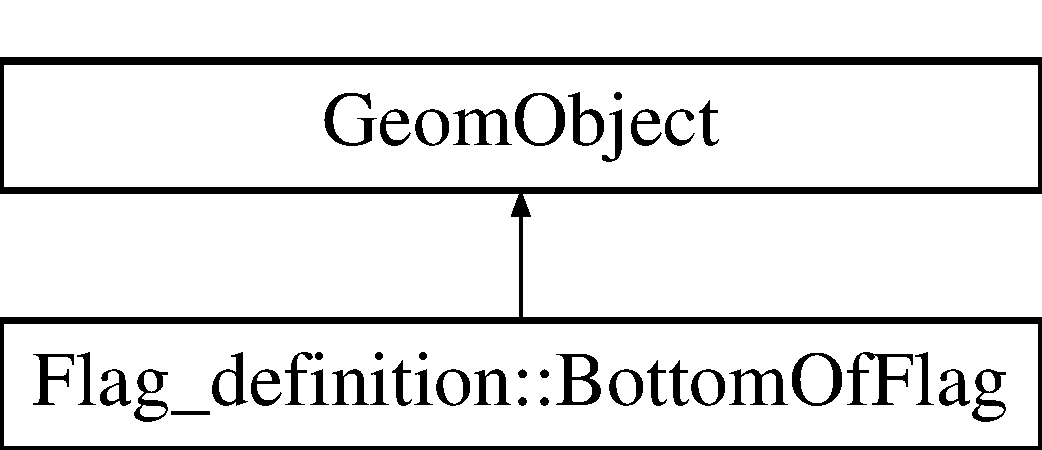
\includegraphics[height=2.000000cm]{classFlag__definition_1_1BottomOfFlag}
\end{center}
\end{figure}
\subsection*{Public Member Functions}
\begin{DoxyCompactItemize}
\item 
\hyperlink{classFlag__definition_1_1BottomOfFlag_a5433f7ea42d0ac1c8eef2c1d65f070de}{Bottom\+Of\+Flag} ()
\begin{DoxyCompactList}\small\item\em Constructor\+: \end{DoxyCompactList}\item 
\hyperlink{classFlag__definition_1_1BottomOfFlag_ab3689967f7beab309822c4a4d9b59f32}{$\sim$\+Bottom\+Of\+Flag} ()
\begin{DoxyCompactList}\small\item\em Destructor (empty) \end{DoxyCompactList}\item 
void \hyperlink{classFlag__definition_1_1BottomOfFlag_a3d3054be363af2acfeca9769bd7c6684}{position} (const unsigned \&t, const Vector$<$ double $>$ \&xi, Vector$<$ double $>$ \&r) const
\begin{DoxyCompactList}\small\item\em Return the position along the bottom of the flag (xi\mbox{[}0\mbox{]} varies between 0 and Lx) \end{DoxyCompactList}\item 
void \hyperlink{classFlag__definition_1_1BottomOfFlag_aa534848e399e6fa14a279ec45142df87}{position} (const Vector$<$ double $>$ \&xi, Vector$<$ double $>$ \&r) const
\begin{DoxyCompactList}\small\item\em Current position. \end{DoxyCompactList}\item 
unsigned \hyperlink{classFlag__definition_1_1BottomOfFlag_a7aba815793bcc775d97b6be533ff6b44}{ngeom\+\_\+data} () const
\begin{DoxyCompactList}\small\item\em Number of geometric Data in Geom\+Object\+: None. \end{DoxyCompactList}\end{DoxyCompactItemize}


\subsection{Detailed Description}
Geom\+Object that defines the lower boundary of the flag. 

Definition at line 180 of file turek\+\_\+flag\+\_\+non\+\_\+fsi.\+cc.



\subsection{Constructor \& Destructor Documentation}
\mbox{\Hypertarget{classFlag__definition_1_1BottomOfFlag_a5433f7ea42d0ac1c8eef2c1d65f070de}\label{classFlag__definition_1_1BottomOfFlag_a5433f7ea42d0ac1c8eef2c1d65f070de}} 
\index{Flag\+\_\+definition\+::\+Bottom\+Of\+Flag@{Flag\+\_\+definition\+::\+Bottom\+Of\+Flag}!Bottom\+Of\+Flag@{Bottom\+Of\+Flag}}
\index{Bottom\+Of\+Flag@{Bottom\+Of\+Flag}!Flag\+\_\+definition\+::\+Bottom\+Of\+Flag@{Flag\+\_\+definition\+::\+Bottom\+Of\+Flag}}
\subsubsection{\texorpdfstring{Bottom\+Of\+Flag()}{BottomOfFlag()}}
{\footnotesize\ttfamily Flag\+\_\+definition\+::\+Bottom\+Of\+Flag\+::\+Bottom\+Of\+Flag (\begin{DoxyParamCaption}{ }\end{DoxyParamCaption})\hspace{0.3cm}{\ttfamily [inline]}}



Constructor\+: 



Definition at line 186 of file turek\+\_\+flag\+\_\+non\+\_\+fsi.\+cc.

\mbox{\Hypertarget{classFlag__definition_1_1BottomOfFlag_ab3689967f7beab309822c4a4d9b59f32}\label{classFlag__definition_1_1BottomOfFlag_ab3689967f7beab309822c4a4d9b59f32}} 
\index{Flag\+\_\+definition\+::\+Bottom\+Of\+Flag@{Flag\+\_\+definition\+::\+Bottom\+Of\+Flag}!````~Bottom\+Of\+Flag@{$\sim$\+Bottom\+Of\+Flag}}
\index{````~Bottom\+Of\+Flag@{$\sim$\+Bottom\+Of\+Flag}!Flag\+\_\+definition\+::\+Bottom\+Of\+Flag@{Flag\+\_\+definition\+::\+Bottom\+Of\+Flag}}
\subsubsection{\texorpdfstring{$\sim$\+Bottom\+Of\+Flag()}{~BottomOfFlag()}}
{\footnotesize\ttfamily Flag\+\_\+definition\+::\+Bottom\+Of\+Flag\+::$\sim$\+Bottom\+Of\+Flag (\begin{DoxyParamCaption}{ }\end{DoxyParamCaption})\hspace{0.3cm}{\ttfamily [inline]}}



Destructor (empty) 



Definition at line 189 of file turek\+\_\+flag\+\_\+non\+\_\+fsi.\+cc.



\subsection{Member Function Documentation}
\mbox{\Hypertarget{classFlag__definition_1_1BottomOfFlag_a7aba815793bcc775d97b6be533ff6b44}\label{classFlag__definition_1_1BottomOfFlag_a7aba815793bcc775d97b6be533ff6b44}} 
\index{Flag\+\_\+definition\+::\+Bottom\+Of\+Flag@{Flag\+\_\+definition\+::\+Bottom\+Of\+Flag}!ngeom\+\_\+data@{ngeom\+\_\+data}}
\index{ngeom\+\_\+data@{ngeom\+\_\+data}!Flag\+\_\+definition\+::\+Bottom\+Of\+Flag@{Flag\+\_\+definition\+::\+Bottom\+Of\+Flag}}
\subsubsection{\texorpdfstring{ngeom\+\_\+data()}{ngeom\_data()}}
{\footnotesize\ttfamily unsigned Flag\+\_\+definition\+::\+Bottom\+Of\+Flag\+::ngeom\+\_\+data (\begin{DoxyParamCaption}{ }\end{DoxyParamCaption}) const\hspace{0.3cm}{\ttfamily [inline]}}



Number of geometric Data in Geom\+Object\+: None. 



Definition at line 221 of file turek\+\_\+flag\+\_\+non\+\_\+fsi.\+cc.

\mbox{\Hypertarget{classFlag__definition_1_1BottomOfFlag_a3d3054be363af2acfeca9769bd7c6684}\label{classFlag__definition_1_1BottomOfFlag_a3d3054be363af2acfeca9769bd7c6684}} 
\index{Flag\+\_\+definition\+::\+Bottom\+Of\+Flag@{Flag\+\_\+definition\+::\+Bottom\+Of\+Flag}!position@{position}}
\index{position@{position}!Flag\+\_\+definition\+::\+Bottom\+Of\+Flag@{Flag\+\_\+definition\+::\+Bottom\+Of\+Flag}}
\subsubsection{\texorpdfstring{position()}{position()}\hspace{0.1cm}{\footnotesize\ttfamily [1/2]}}
{\footnotesize\ttfamily void Flag\+\_\+definition\+::\+Bottom\+Of\+Flag\+::position (\begin{DoxyParamCaption}\item[{const unsigned \&}]{t,  }\item[{const Vector$<$ double $>$ \&}]{xi,  }\item[{Vector$<$ double $>$ \&}]{r }\end{DoxyParamCaption}) const\hspace{0.3cm}{\ttfamily [inline]}}



Return the position along the bottom of the flag (xi\mbox{[}0\mbox{]} varies between 0 and Lx) 



Definition at line 194 of file turek\+\_\+flag\+\_\+non\+\_\+fsi.\+cc.



References Flag\+\_\+definition\+::lower\+\_\+tip(), and Flag\+\_\+definition\+::\+Period.

\mbox{\Hypertarget{classFlag__definition_1_1BottomOfFlag_aa534848e399e6fa14a279ec45142df87}\label{classFlag__definition_1_1BottomOfFlag_aa534848e399e6fa14a279ec45142df87}} 
\index{Flag\+\_\+definition\+::\+Bottom\+Of\+Flag@{Flag\+\_\+definition\+::\+Bottom\+Of\+Flag}!position@{position}}
\index{position@{position}!Flag\+\_\+definition\+::\+Bottom\+Of\+Flag@{Flag\+\_\+definition\+::\+Bottom\+Of\+Flag}}
\subsubsection{\texorpdfstring{position()}{position()}\hspace{0.1cm}{\footnotesize\ttfamily [2/2]}}
{\footnotesize\ttfamily void Flag\+\_\+definition\+::\+Bottom\+Of\+Flag\+::position (\begin{DoxyParamCaption}\item[{const Vector$<$ double $>$ \&}]{xi,  }\item[{Vector$<$ double $>$ \&}]{r }\end{DoxyParamCaption}) const\hspace{0.3cm}{\ttfamily [inline]}}



Current position. 



Definition at line 215 of file turek\+\_\+flag\+\_\+non\+\_\+fsi.\+cc.



The documentation for this class was generated from the following file\+:\begin{DoxyCompactItemize}
\item 
\hyperlink{turek__flag__non__fsi_8cc}{turek\+\_\+flag\+\_\+non\+\_\+fsi.\+cc}\end{DoxyCompactItemize}

\hypertarget{classFlag__definition_1_1TipOfFlag}{}\section{Flag\+\_\+definition\+:\+:Tip\+Of\+Flag Class Reference}
\label{classFlag__definition_1_1TipOfFlag}\index{Flag\+\_\+definition\+::\+Tip\+Of\+Flag@{Flag\+\_\+definition\+::\+Tip\+Of\+Flag}}


Geom\+Object that defines the tip of the flag.  


Inheritance diagram for Flag\+\_\+definition\+:\+:Tip\+Of\+Flag\+:\begin{figure}[H]
\begin{center}
\leavevmode
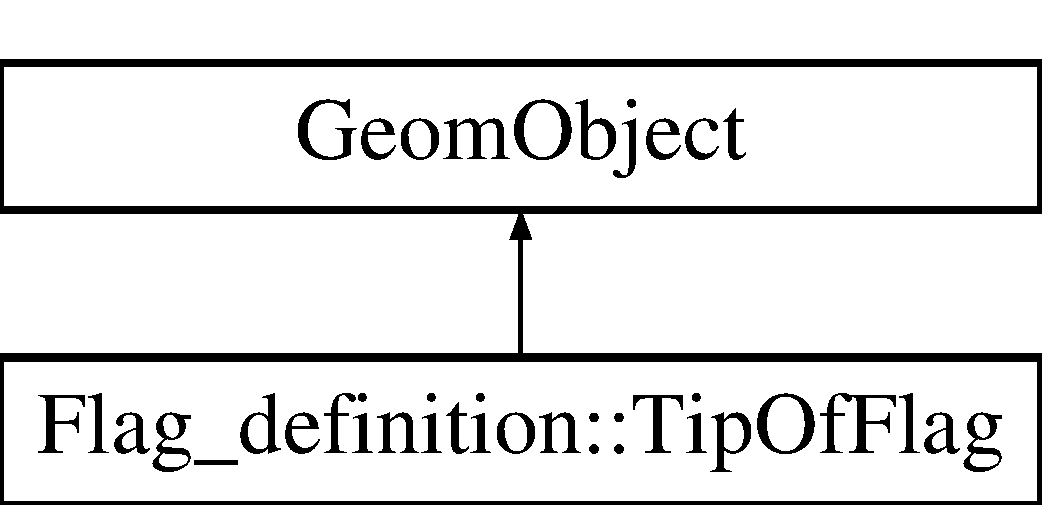
\includegraphics[height=2.000000cm]{classFlag__definition_1_1TipOfFlag}
\end{center}
\end{figure}
\subsection*{Public Member Functions}
\begin{DoxyCompactItemize}
\item 
\hyperlink{classFlag__definition_1_1TipOfFlag_a7a43bdfc369a833e161a75d29b95ff01}{Tip\+Of\+Flag} ()
\begin{DoxyCompactList}\small\item\em Constructor. \end{DoxyCompactList}\item 
\hyperlink{classFlag__definition_1_1TipOfFlag_a9aa1a8091a79925dc6542ab2c03d583a}{$\sim$\+Tip\+Of\+Flag} ()
\begin{DoxyCompactList}\small\item\em Destructor (empty) \end{DoxyCompactList}\item 
void \hyperlink{classFlag__definition_1_1TipOfFlag_afcc0a2176290bbb7d1bb4adf9c231991}{position} (const unsigned \&t, const Vector$<$ double $>$ \&xi, Vector$<$ double $>$ \&r) const
\begin{DoxyCompactList}\small\item\em Return the position This object links the tips of the top and bottom by a straight line whilst xi\mbox{[}0\mbox{]} goes from -\/\+H/2 to H/2. \end{DoxyCompactList}\item 
void \hyperlink{classFlag__definition_1_1TipOfFlag_ae4e08c72baeaca1fe62bca6f36262fa7}{position} (const Vector$<$ double $>$ \&xi, Vector$<$ double $>$ \&r) const
\begin{DoxyCompactList}\small\item\em Current position. \end{DoxyCompactList}\item 
unsigned \hyperlink{classFlag__definition_1_1TipOfFlag_a7571a5cbebe6de6c4ee42de5f2fe3dd8}{ngeom\+\_\+data} () const
\begin{DoxyCompactList}\small\item\em Number of geometric Data in Geom\+Object\+: None. \end{DoxyCompactList}\end{DoxyCompactItemize}


\subsection{Detailed Description}
Geom\+Object that defines the tip of the flag. 

Definition at line 231 of file turek\+\_\+flag\+\_\+non\+\_\+fsi.\+cc.



\subsection{Constructor \& Destructor Documentation}
\mbox{\Hypertarget{classFlag__definition_1_1TipOfFlag_a7a43bdfc369a833e161a75d29b95ff01}\label{classFlag__definition_1_1TipOfFlag_a7a43bdfc369a833e161a75d29b95ff01}} 
\index{Flag\+\_\+definition\+::\+Tip\+Of\+Flag@{Flag\+\_\+definition\+::\+Tip\+Of\+Flag}!Tip\+Of\+Flag@{Tip\+Of\+Flag}}
\index{Tip\+Of\+Flag@{Tip\+Of\+Flag}!Flag\+\_\+definition\+::\+Tip\+Of\+Flag@{Flag\+\_\+definition\+::\+Tip\+Of\+Flag}}
\subsubsection{\texorpdfstring{Tip\+Of\+Flag()}{TipOfFlag()}}
{\footnotesize\ttfamily Flag\+\_\+definition\+::\+Tip\+Of\+Flag\+::\+Tip\+Of\+Flag (\begin{DoxyParamCaption}{ }\end{DoxyParamCaption})\hspace{0.3cm}{\ttfamily [inline]}}



Constructor. 



Definition at line 237 of file turek\+\_\+flag\+\_\+non\+\_\+fsi.\+cc.

\mbox{\Hypertarget{classFlag__definition_1_1TipOfFlag_a9aa1a8091a79925dc6542ab2c03d583a}\label{classFlag__definition_1_1TipOfFlag_a9aa1a8091a79925dc6542ab2c03d583a}} 
\index{Flag\+\_\+definition\+::\+Tip\+Of\+Flag@{Flag\+\_\+definition\+::\+Tip\+Of\+Flag}!````~Tip\+Of\+Flag@{$\sim$\+Tip\+Of\+Flag}}
\index{````~Tip\+Of\+Flag@{$\sim$\+Tip\+Of\+Flag}!Flag\+\_\+definition\+::\+Tip\+Of\+Flag@{Flag\+\_\+definition\+::\+Tip\+Of\+Flag}}
\subsubsection{\texorpdfstring{$\sim$\+Tip\+Of\+Flag()}{~TipOfFlag()}}
{\footnotesize\ttfamily Flag\+\_\+definition\+::\+Tip\+Of\+Flag\+::$\sim$\+Tip\+Of\+Flag (\begin{DoxyParamCaption}{ }\end{DoxyParamCaption})\hspace{0.3cm}{\ttfamily [inline]}}



Destructor (empty) 



Definition at line 240 of file turek\+\_\+flag\+\_\+non\+\_\+fsi.\+cc.



\subsection{Member Function Documentation}
\mbox{\Hypertarget{classFlag__definition_1_1TipOfFlag_a7571a5cbebe6de6c4ee42de5f2fe3dd8}\label{classFlag__definition_1_1TipOfFlag_a7571a5cbebe6de6c4ee42de5f2fe3dd8}} 
\index{Flag\+\_\+definition\+::\+Tip\+Of\+Flag@{Flag\+\_\+definition\+::\+Tip\+Of\+Flag}!ngeom\+\_\+data@{ngeom\+\_\+data}}
\index{ngeom\+\_\+data@{ngeom\+\_\+data}!Flag\+\_\+definition\+::\+Tip\+Of\+Flag@{Flag\+\_\+definition\+::\+Tip\+Of\+Flag}}
\subsubsection{\texorpdfstring{ngeom\+\_\+data()}{ngeom\_data()}}
{\footnotesize\ttfamily unsigned Flag\+\_\+definition\+::\+Tip\+Of\+Flag\+::ngeom\+\_\+data (\begin{DoxyParamCaption}{ }\end{DoxyParamCaption}) const\hspace{0.3cm}{\ttfamily [inline]}}



Number of geometric Data in Geom\+Object\+: None. 



Definition at line 262 of file turek\+\_\+flag\+\_\+non\+\_\+fsi.\+cc.

\mbox{\Hypertarget{classFlag__definition_1_1TipOfFlag_afcc0a2176290bbb7d1bb4adf9c231991}\label{classFlag__definition_1_1TipOfFlag_afcc0a2176290bbb7d1bb4adf9c231991}} 
\index{Flag\+\_\+definition\+::\+Tip\+Of\+Flag@{Flag\+\_\+definition\+::\+Tip\+Of\+Flag}!position@{position}}
\index{position@{position}!Flag\+\_\+definition\+::\+Tip\+Of\+Flag@{Flag\+\_\+definition\+::\+Tip\+Of\+Flag}}
\subsubsection{\texorpdfstring{position()}{position()}\hspace{0.1cm}{\footnotesize\ttfamily [1/2]}}
{\footnotesize\ttfamily void Flag\+\_\+definition\+::\+Tip\+Of\+Flag\+::position (\begin{DoxyParamCaption}\item[{const unsigned \&}]{t,  }\item[{const Vector$<$ double $>$ \&}]{xi,  }\item[{Vector$<$ double $>$ \&}]{r }\end{DoxyParamCaption}) const\hspace{0.3cm}{\ttfamily [inline]}}



Return the position This object links the tips of the top and bottom by a straight line whilst xi\mbox{[}0\mbox{]} goes from -\/\+H/2 to H/2. 



Definition at line 245 of file turek\+\_\+flag\+\_\+non\+\_\+fsi.\+cc.



References Flag\+\_\+definition\+::lower\+\_\+tip(), and Flag\+\_\+definition\+::upper\+\_\+tip().

\mbox{\Hypertarget{classFlag__definition_1_1TipOfFlag_ae4e08c72baeaca1fe62bca6f36262fa7}\label{classFlag__definition_1_1TipOfFlag_ae4e08c72baeaca1fe62bca6f36262fa7}} 
\index{Flag\+\_\+definition\+::\+Tip\+Of\+Flag@{Flag\+\_\+definition\+::\+Tip\+Of\+Flag}!position@{position}}
\index{position@{position}!Flag\+\_\+definition\+::\+Tip\+Of\+Flag@{Flag\+\_\+definition\+::\+Tip\+Of\+Flag}}
\subsubsection{\texorpdfstring{position()}{position()}\hspace{0.1cm}{\footnotesize\ttfamily [2/2]}}
{\footnotesize\ttfamily void Flag\+\_\+definition\+::\+Tip\+Of\+Flag\+::position (\begin{DoxyParamCaption}\item[{const Vector$<$ double $>$ \&}]{xi,  }\item[{Vector$<$ double $>$ \&}]{r }\end{DoxyParamCaption}) const\hspace{0.3cm}{\ttfamily [inline]}}



Current position. 



Definition at line 256 of file turek\+\_\+flag\+\_\+non\+\_\+fsi.\+cc.



The documentation for this class was generated from the following file\+:\begin{DoxyCompactItemize}
\item 
\hyperlink{turek__flag__non__fsi_8cc}{turek\+\_\+flag\+\_\+non\+\_\+fsi.\+cc}\end{DoxyCompactItemize}

\hypertarget{classFlag__definition_1_1TopOfFlag}{}\section{Flag\+\_\+definition\+:\+:Top\+Of\+Flag Class Reference}
\label{classFlag__definition_1_1TopOfFlag}\index{Flag\+\_\+definition\+::\+Top\+Of\+Flag@{Flag\+\_\+definition\+::\+Top\+Of\+Flag}}


Geom\+Object that defines the upper boundary of the flag.  


Inheritance diagram for Flag\+\_\+definition\+:\+:Top\+Of\+Flag\+:\begin{figure}[H]
\begin{center}
\leavevmode
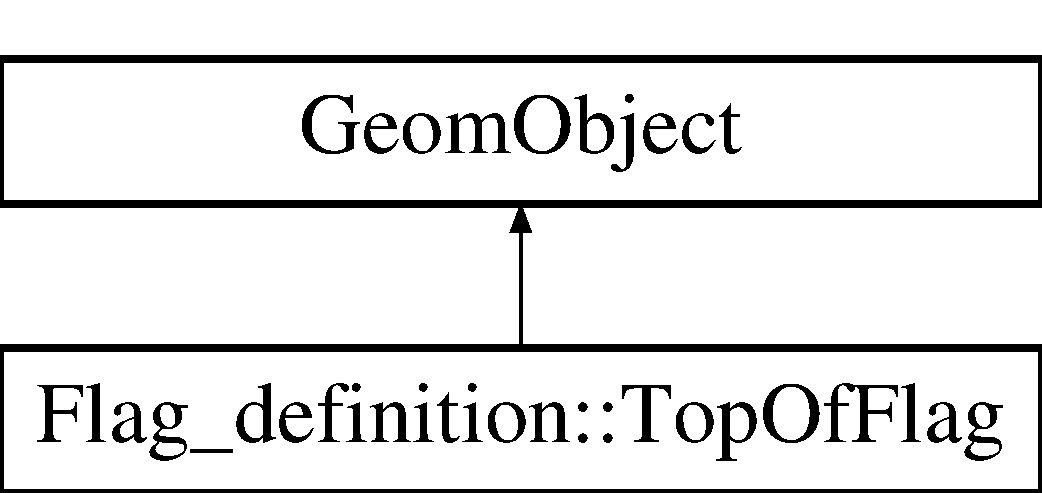
\includegraphics[height=2.000000cm]{classFlag__definition_1_1TopOfFlag}
\end{center}
\end{figure}
\subsection*{Public Member Functions}
\begin{DoxyCompactItemize}
\item 
\hyperlink{classFlag__definition_1_1TopOfFlag_a187ed8b664190ab0feb971198d74ff2b}{Top\+Of\+Flag} ()
\begin{DoxyCompactList}\small\item\em Constructor\+: It\textquotesingle{}s a 1D object in 2D space. \end{DoxyCompactList}\item 
\hyperlink{classFlag__definition_1_1TopOfFlag_ab2f5971dfc14401c536ede9006da7c8a}{$\sim$\+Top\+Of\+Flag} ()
\begin{DoxyCompactList}\small\item\em Destructor (empty) \end{DoxyCompactList}\item 
void \hyperlink{classFlag__definition_1_1TopOfFlag_a99adccd501bc69e0af51918d77e0f1b7}{position} (const unsigned \&t, const Vector$<$ double $>$ \&xi, Vector$<$ double $>$ \&r) const
\begin{DoxyCompactList}\small\item\em Return the position along the top of the flag (xi\mbox{[}0\mbox{]} varies between 0 and Lx) \end{DoxyCompactList}\item 
void \hyperlink{classFlag__definition_1_1TopOfFlag_a0a902ee453f96231b41aa66e3c3b8bf0}{position} (const Vector$<$ double $>$ \&xi, Vector$<$ double $>$ \&r) const
\begin{DoxyCompactList}\small\item\em Current position. \end{DoxyCompactList}\item 
unsigned \hyperlink{classFlag__definition_1_1TopOfFlag_a1ca5543c07da97885e955acd241616ec}{ngeom\+\_\+data} () const
\begin{DoxyCompactList}\small\item\em Number of geometric Data in Geom\+Object\+: None. \end{DoxyCompactList}\end{DoxyCompactItemize}


\subsection{Detailed Description}
Geom\+Object that defines the upper boundary of the flag. 

Definition at line 130 of file turek\+\_\+flag\+\_\+non\+\_\+fsi.\+cc.



\subsection{Constructor \& Destructor Documentation}
\mbox{\Hypertarget{classFlag__definition_1_1TopOfFlag_a187ed8b664190ab0feb971198d74ff2b}\label{classFlag__definition_1_1TopOfFlag_a187ed8b664190ab0feb971198d74ff2b}} 
\index{Flag\+\_\+definition\+::\+Top\+Of\+Flag@{Flag\+\_\+definition\+::\+Top\+Of\+Flag}!Top\+Of\+Flag@{Top\+Of\+Flag}}
\index{Top\+Of\+Flag@{Top\+Of\+Flag}!Flag\+\_\+definition\+::\+Top\+Of\+Flag@{Flag\+\_\+definition\+::\+Top\+Of\+Flag}}
\subsubsection{\texorpdfstring{Top\+Of\+Flag()}{TopOfFlag()}}
{\footnotesize\ttfamily Flag\+\_\+definition\+::\+Top\+Of\+Flag\+::\+Top\+Of\+Flag (\begin{DoxyParamCaption}{ }\end{DoxyParamCaption})\hspace{0.3cm}{\ttfamily [inline]}}



Constructor\+: It\textquotesingle{}s a 1D object in 2D space. 



Definition at line 136 of file turek\+\_\+flag\+\_\+non\+\_\+fsi.\+cc.

\mbox{\Hypertarget{classFlag__definition_1_1TopOfFlag_ab2f5971dfc14401c536ede9006da7c8a}\label{classFlag__definition_1_1TopOfFlag_ab2f5971dfc14401c536ede9006da7c8a}} 
\index{Flag\+\_\+definition\+::\+Top\+Of\+Flag@{Flag\+\_\+definition\+::\+Top\+Of\+Flag}!````~Top\+Of\+Flag@{$\sim$\+Top\+Of\+Flag}}
\index{````~Top\+Of\+Flag@{$\sim$\+Top\+Of\+Flag}!Flag\+\_\+definition\+::\+Top\+Of\+Flag@{Flag\+\_\+definition\+::\+Top\+Of\+Flag}}
\subsubsection{\texorpdfstring{$\sim$\+Top\+Of\+Flag()}{~TopOfFlag()}}
{\footnotesize\ttfamily Flag\+\_\+definition\+::\+Top\+Of\+Flag\+::$\sim$\+Top\+Of\+Flag (\begin{DoxyParamCaption}{ }\end{DoxyParamCaption})\hspace{0.3cm}{\ttfamily [inline]}}



Destructor (empty) 



Definition at line 139 of file turek\+\_\+flag\+\_\+non\+\_\+fsi.\+cc.



\subsection{Member Function Documentation}
\mbox{\Hypertarget{classFlag__definition_1_1TopOfFlag_a1ca5543c07da97885e955acd241616ec}\label{classFlag__definition_1_1TopOfFlag_a1ca5543c07da97885e955acd241616ec}} 
\index{Flag\+\_\+definition\+::\+Top\+Of\+Flag@{Flag\+\_\+definition\+::\+Top\+Of\+Flag}!ngeom\+\_\+data@{ngeom\+\_\+data}}
\index{ngeom\+\_\+data@{ngeom\+\_\+data}!Flag\+\_\+definition\+::\+Top\+Of\+Flag@{Flag\+\_\+definition\+::\+Top\+Of\+Flag}}
\subsubsection{\texorpdfstring{ngeom\+\_\+data()}{ngeom\_data()}}
{\footnotesize\ttfamily unsigned Flag\+\_\+definition\+::\+Top\+Of\+Flag\+::ngeom\+\_\+data (\begin{DoxyParamCaption}{ }\end{DoxyParamCaption}) const\hspace{0.3cm}{\ttfamily [inline]}}



Number of geometric Data in Geom\+Object\+: None. 



Definition at line 171 of file turek\+\_\+flag\+\_\+non\+\_\+fsi.\+cc.

\mbox{\Hypertarget{classFlag__definition_1_1TopOfFlag_a99adccd501bc69e0af51918d77e0f1b7}\label{classFlag__definition_1_1TopOfFlag_a99adccd501bc69e0af51918d77e0f1b7}} 
\index{Flag\+\_\+definition\+::\+Top\+Of\+Flag@{Flag\+\_\+definition\+::\+Top\+Of\+Flag}!position@{position}}
\index{position@{position}!Flag\+\_\+definition\+::\+Top\+Of\+Flag@{Flag\+\_\+definition\+::\+Top\+Of\+Flag}}
\subsubsection{\texorpdfstring{position()}{position()}\hspace{0.1cm}{\footnotesize\ttfamily [1/2]}}
{\footnotesize\ttfamily void Flag\+\_\+definition\+::\+Top\+Of\+Flag\+::position (\begin{DoxyParamCaption}\item[{const unsigned \&}]{t,  }\item[{const Vector$<$ double $>$ \&}]{xi,  }\item[{Vector$<$ double $>$ \&}]{r }\end{DoxyParamCaption}) const\hspace{0.3cm}{\ttfamily [inline]}}



Return the position along the top of the flag (xi\mbox{[}0\mbox{]} varies between 0 and Lx) 



Definition at line 143 of file turek\+\_\+flag\+\_\+non\+\_\+fsi.\+cc.



References Flag\+\_\+definition\+::\+Period, and Flag\+\_\+definition\+::upper\+\_\+tip().

\mbox{\Hypertarget{classFlag__definition_1_1TopOfFlag_a0a902ee453f96231b41aa66e3c3b8bf0}\label{classFlag__definition_1_1TopOfFlag_a0a902ee453f96231b41aa66e3c3b8bf0}} 
\index{Flag\+\_\+definition\+::\+Top\+Of\+Flag@{Flag\+\_\+definition\+::\+Top\+Of\+Flag}!position@{position}}
\index{position@{position}!Flag\+\_\+definition\+::\+Top\+Of\+Flag@{Flag\+\_\+definition\+::\+Top\+Of\+Flag}}
\subsubsection{\texorpdfstring{position()}{position()}\hspace{0.1cm}{\footnotesize\ttfamily [2/2]}}
{\footnotesize\ttfamily void Flag\+\_\+definition\+::\+Top\+Of\+Flag\+::position (\begin{DoxyParamCaption}\item[{const Vector$<$ double $>$ \&}]{xi,  }\item[{Vector$<$ double $>$ \&}]{r }\end{DoxyParamCaption}) const\hspace{0.3cm}{\ttfamily [inline]}}



Current position. 



Definition at line 165 of file turek\+\_\+flag\+\_\+non\+\_\+fsi.\+cc.



The documentation for this class was generated from the following file\+:\begin{DoxyCompactItemize}
\item 
\hyperlink{turek__flag__non__fsi_8cc}{turek\+\_\+flag\+\_\+non\+\_\+fsi.\+cc}\end{DoxyCompactItemize}

\hypertarget{classTurekNonFSIProblem}{}\section{Turek\+Non\+F\+S\+I\+Problem$<$ E\+L\+E\+M\+E\+NT $>$ Class Template Reference}
\label{classTurekNonFSIProblem}\index{Turek\+Non\+F\+S\+I\+Problem$<$ E\+L\+E\+M\+E\+N\+T $>$@{Turek\+Non\+F\+S\+I\+Problem$<$ E\+L\+E\+M\+E\+N\+T $>$}}


Flow around a cylinder with flag.  


Inheritance diagram for Turek\+Non\+F\+S\+I\+Problem$<$ E\+L\+E\+M\+E\+NT $>$\+:\begin{figure}[H]
\begin{center}
\leavevmode
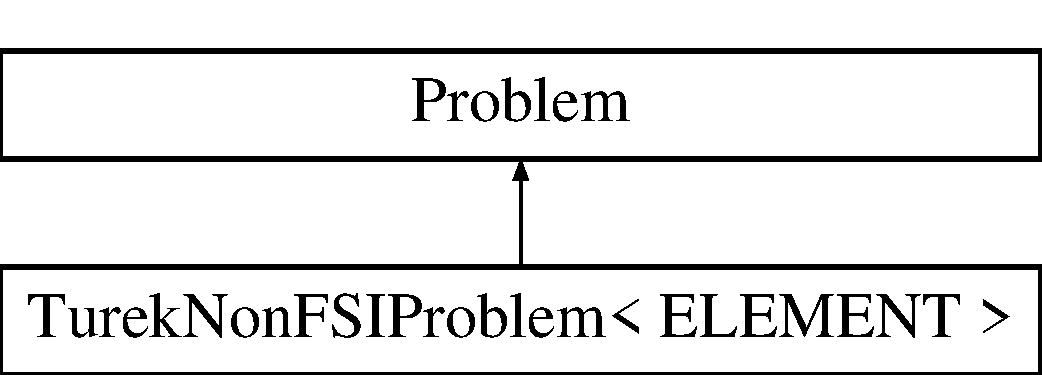
\includegraphics[height=2.000000cm]{classTurekNonFSIProblem}
\end{center}
\end{figure}
\subsection*{Public Member Functions}
\begin{DoxyCompactItemize}
\item 
\hyperlink{classTurekNonFSIProblem_aacb3214544ef81c2f8b49777457e8be6}{Turek\+Non\+F\+S\+I\+Problem} (const double \&length, const double \&height)
\begin{DoxyCompactList}\small\item\em Constructor\+: Pass length and height of domain. \end{DoxyCompactList}\item 
void \hyperlink{classTurekNonFSIProblem_a161cfe46817a5129dcc33c7ce3a17173}{actions\+\_\+after\+\_\+newton\+\_\+solve} ()
\begin{DoxyCompactList}\small\item\em Update the problem specs after solve (empty) \end{DoxyCompactList}\item 
void \hyperlink{classTurekNonFSIProblem_ae5881b3424aee1ba7b947fff96493d2f}{actions\+\_\+before\+\_\+newton\+\_\+solve} ()
\begin{DoxyCompactList}\small\item\em Update the problem specs before solve (empty) \end{DoxyCompactList}\item 
void \hyperlink{classTurekNonFSIProblem_a88ed5ef8b1be34f5176c29ffec20eedd}{actions\+\_\+after\+\_\+adapt} ()
\begin{DoxyCompactList}\small\item\em After adaptation\+: Unpin pressures and pin redudant pressure dofs. \end{DoxyCompactList}\item 
void \hyperlink{classTurekNonFSIProblem_a29725cde9071c3a83792469787ea6c7d}{actions\+\_\+before\+\_\+implicit\+\_\+timestep} ()
\begin{DoxyCompactList}\small\item\em Update the velocity boundary condition on the flag. \end{DoxyCompactList}\item 
Refineable\+Cylinder\+With\+Flag\+Mesh$<$ E\+L\+E\+M\+E\+NT $>$ $\ast$ \hyperlink{classTurekNonFSIProblem_a6b9af904a3091d55a61b35c2ce7d7fcb}{mesh\+\_\+pt} ()
\begin{DoxyCompactList}\small\item\em Access function for the specific mesh. \end{DoxyCompactList}\item 
Refineable\+Algebraic\+Cylinder\+With\+Flag\+Mesh$<$ E\+L\+E\+M\+E\+NT $>$ $\ast$ \hyperlink{classTurekNonFSIProblem_a46da5ab0ac3d390eba02f7a4eb2795d5}{mesh\+\_\+pt} ()
\begin{DoxyCompactList}\small\item\em Access function for the specific mesh. \end{DoxyCompactList}\item 
void \hyperlink{classTurekNonFSIProblem_a2f129e4eba71784a58b27d846fdc2a61}{doc\+\_\+solution} (Doc\+Info \&doc\+\_\+info)
\begin{DoxyCompactList}\small\item\em Doc the solution. \end{DoxyCompactList}\end{DoxyCompactItemize}
\subsection*{Private Attributes}
\begin{DoxyCompactItemize}
\item 
double \hyperlink{classTurekNonFSIProblem_a7e85e76876a9b1136cc340b0bb25e299}{Height}
\begin{DoxyCompactList}\small\item\em Height of channel. \end{DoxyCompactList}\end{DoxyCompactItemize}


\subsection{Detailed Description}
\subsubsection*{template$<$class E\+L\+E\+M\+E\+NT$>$\newline
class Turek\+Non\+F\+S\+I\+Problem$<$ E\+L\+E\+M\+E\+N\+T $>$}

Flow around a cylinder with flag. 

Definition at line 315 of file turek\+\_\+flag\+\_\+non\+\_\+fsi.\+cc.



\subsection{Constructor \& Destructor Documentation}
\mbox{\Hypertarget{classTurekNonFSIProblem_aacb3214544ef81c2f8b49777457e8be6}\label{classTurekNonFSIProblem_aacb3214544ef81c2f8b49777457e8be6}} 
\index{Turek\+Non\+F\+S\+I\+Problem@{Turek\+Non\+F\+S\+I\+Problem}!Turek\+Non\+F\+S\+I\+Problem@{Turek\+Non\+F\+S\+I\+Problem}}
\index{Turek\+Non\+F\+S\+I\+Problem@{Turek\+Non\+F\+S\+I\+Problem}!Turek\+Non\+F\+S\+I\+Problem@{Turek\+Non\+F\+S\+I\+Problem}}
\subsubsection{\texorpdfstring{Turek\+Non\+F\+S\+I\+Problem()}{TurekNonFSIProblem()}}
{\footnotesize\ttfamily template$<$class E\+L\+E\+M\+E\+NT $>$ \\
\hyperlink{classTurekNonFSIProblem}{Turek\+Non\+F\+S\+I\+Problem}$<$ E\+L\+E\+M\+E\+NT $>$\+::\hyperlink{classTurekNonFSIProblem}{Turek\+Non\+F\+S\+I\+Problem} (\begin{DoxyParamCaption}\item[{const double \&}]{length,  }\item[{const double \&}]{height }\end{DoxyParamCaption})}



Constructor\+: Pass length and height of domain. 



Definition at line 375 of file turek\+\_\+flag\+\_\+non\+\_\+fsi.\+cc.



References Flag\+\_\+definition\+::\+Bottom\+\_\+flag\+\_\+pt, Flag\+\_\+definition\+::\+Centre\+\_\+x, Flag\+\_\+definition\+::\+Centre\+\_\+y, Flag\+\_\+definition\+::\+Cylinder\+\_\+pt, Flag\+\_\+definition\+::H, Turek\+Non\+F\+S\+I\+Problem$<$ E\+L\+E\+M\+E\+N\+T $>$\+::\+Height, Flag\+\_\+definition\+::L, Turek\+Non\+F\+S\+I\+Problem$<$ E\+L\+E\+M\+E\+N\+T $>$\+::mesh\+\_\+pt(), Flag\+\_\+definition\+::\+Radius, Global\+\_\+\+Parameters\+::\+Re, Flag\+\_\+definition\+::setup(), Flag\+\_\+definition\+::\+Tip\+\_\+flag\+\_\+pt, and Flag\+\_\+definition\+::\+Top\+\_\+flag\+\_\+pt.



\subsection{Member Function Documentation}
\mbox{\Hypertarget{classTurekNonFSIProblem_a88ed5ef8b1be34f5176c29ffec20eedd}\label{classTurekNonFSIProblem_a88ed5ef8b1be34f5176c29ffec20eedd}} 
\index{Turek\+Non\+F\+S\+I\+Problem@{Turek\+Non\+F\+S\+I\+Problem}!actions\+\_\+after\+\_\+adapt@{actions\+\_\+after\+\_\+adapt}}
\index{actions\+\_\+after\+\_\+adapt@{actions\+\_\+after\+\_\+adapt}!Turek\+Non\+F\+S\+I\+Problem@{Turek\+Non\+F\+S\+I\+Problem}}
\subsubsection{\texorpdfstring{actions\+\_\+after\+\_\+adapt()}{actions\_after\_adapt()}}
{\footnotesize\ttfamily template$<$class E\+L\+E\+M\+E\+NT $>$ \\
void \hyperlink{classTurekNonFSIProblem}{Turek\+Non\+F\+S\+I\+Problem}$<$ E\+L\+E\+M\+E\+NT $>$\+::actions\+\_\+after\+\_\+adapt (\begin{DoxyParamCaption}{ }\end{DoxyParamCaption})}



After adaptation\+: Unpin pressures and pin redudant pressure dofs. 

Actions after adapt. 

Definition at line 507 of file turek\+\_\+flag\+\_\+non\+\_\+fsi.\+cc.



References Turek\+Non\+F\+S\+I\+Problem$<$ E\+L\+E\+M\+E\+N\+T $>$\+::mesh\+\_\+pt().

\mbox{\Hypertarget{classTurekNonFSIProblem_a161cfe46817a5129dcc33c7ce3a17173}\label{classTurekNonFSIProblem_a161cfe46817a5129dcc33c7ce3a17173}} 
\index{Turek\+Non\+F\+S\+I\+Problem@{Turek\+Non\+F\+S\+I\+Problem}!actions\+\_\+after\+\_\+newton\+\_\+solve@{actions\+\_\+after\+\_\+newton\+\_\+solve}}
\index{actions\+\_\+after\+\_\+newton\+\_\+solve@{actions\+\_\+after\+\_\+newton\+\_\+solve}!Turek\+Non\+F\+S\+I\+Problem@{Turek\+Non\+F\+S\+I\+Problem}}
\subsubsection{\texorpdfstring{actions\+\_\+after\+\_\+newton\+\_\+solve()}{actions\_after\_newton\_solve()}}
{\footnotesize\ttfamily template$<$class E\+L\+E\+M\+E\+NT$>$ \\
void \hyperlink{classTurekNonFSIProblem}{Turek\+Non\+F\+S\+I\+Problem}$<$ E\+L\+E\+M\+E\+NT $>$\+::actions\+\_\+after\+\_\+newton\+\_\+solve (\begin{DoxyParamCaption}{ }\end{DoxyParamCaption})\hspace{0.3cm}{\ttfamily [inline]}}



Update the problem specs after solve (empty) 



Definition at line 325 of file turek\+\_\+flag\+\_\+non\+\_\+fsi.\+cc.

\mbox{\Hypertarget{classTurekNonFSIProblem_a29725cde9071c3a83792469787ea6c7d}\label{classTurekNonFSIProblem_a29725cde9071c3a83792469787ea6c7d}} 
\index{Turek\+Non\+F\+S\+I\+Problem@{Turek\+Non\+F\+S\+I\+Problem}!actions\+\_\+before\+\_\+implicit\+\_\+timestep@{actions\+\_\+before\+\_\+implicit\+\_\+timestep}}
\index{actions\+\_\+before\+\_\+implicit\+\_\+timestep@{actions\+\_\+before\+\_\+implicit\+\_\+timestep}!Turek\+Non\+F\+S\+I\+Problem@{Turek\+Non\+F\+S\+I\+Problem}}
\subsubsection{\texorpdfstring{actions\+\_\+before\+\_\+implicit\+\_\+timestep()}{actions\_before\_implicit\_timestep()}}
{\footnotesize\ttfamily template$<$class E\+L\+E\+M\+E\+NT $>$ \\
void \hyperlink{classTurekNonFSIProblem}{Turek\+Non\+F\+S\+I\+Problem}$<$ E\+L\+E\+M\+E\+NT $>$\+::actions\+\_\+before\+\_\+implicit\+\_\+timestep (\begin{DoxyParamCaption}{ }\end{DoxyParamCaption})}



Update the velocity boundary condition on the flag. 

Actions before implicit timestep\+: Update velocity boundary conditions. 

Definition at line 524 of file turek\+\_\+flag\+\_\+non\+\_\+fsi.\+cc.



References Turek\+Non\+F\+S\+I\+Problem$<$ E\+L\+E\+M\+E\+N\+T $>$\+::mesh\+\_\+pt().

\mbox{\Hypertarget{classTurekNonFSIProblem_ae5881b3424aee1ba7b947fff96493d2f}\label{classTurekNonFSIProblem_ae5881b3424aee1ba7b947fff96493d2f}} 
\index{Turek\+Non\+F\+S\+I\+Problem@{Turek\+Non\+F\+S\+I\+Problem}!actions\+\_\+before\+\_\+newton\+\_\+solve@{actions\+\_\+before\+\_\+newton\+\_\+solve}}
\index{actions\+\_\+before\+\_\+newton\+\_\+solve@{actions\+\_\+before\+\_\+newton\+\_\+solve}!Turek\+Non\+F\+S\+I\+Problem@{Turek\+Non\+F\+S\+I\+Problem}}
\subsubsection{\texorpdfstring{actions\+\_\+before\+\_\+newton\+\_\+solve()}{actions\_before\_newton\_solve()}}
{\footnotesize\ttfamily template$<$class E\+L\+E\+M\+E\+NT$>$ \\
void \hyperlink{classTurekNonFSIProblem}{Turek\+Non\+F\+S\+I\+Problem}$<$ E\+L\+E\+M\+E\+NT $>$\+::actions\+\_\+before\+\_\+newton\+\_\+solve (\begin{DoxyParamCaption}{ }\end{DoxyParamCaption})\hspace{0.3cm}{\ttfamily [inline]}}



Update the problem specs before solve (empty) 



Definition at line 328 of file turek\+\_\+flag\+\_\+non\+\_\+fsi.\+cc.

\mbox{\Hypertarget{classTurekNonFSIProblem_a2f129e4eba71784a58b27d846fdc2a61}\label{classTurekNonFSIProblem_a2f129e4eba71784a58b27d846fdc2a61}} 
\index{Turek\+Non\+F\+S\+I\+Problem@{Turek\+Non\+F\+S\+I\+Problem}!doc\+\_\+solution@{doc\+\_\+solution}}
\index{doc\+\_\+solution@{doc\+\_\+solution}!Turek\+Non\+F\+S\+I\+Problem@{Turek\+Non\+F\+S\+I\+Problem}}
\subsubsection{\texorpdfstring{doc\+\_\+solution()}{doc\_solution()}}
{\footnotesize\ttfamily template$<$class E\+L\+E\+M\+E\+NT $>$ \\
void \hyperlink{classTurekNonFSIProblem}{Turek\+Non\+F\+S\+I\+Problem}$<$ E\+L\+E\+M\+E\+NT $>$\+::doc\+\_\+solution (\begin{DoxyParamCaption}\item[{Doc\+Info \&}]{doc\+\_\+info }\end{DoxyParamCaption})}



Doc the solution. 



Definition at line 551 of file turek\+\_\+flag\+\_\+non\+\_\+fsi.\+cc.



References Turek\+Non\+F\+S\+I\+Problem$<$ E\+L\+E\+M\+E\+N\+T $>$\+::mesh\+\_\+pt().

\mbox{\Hypertarget{classTurekNonFSIProblem_a6b9af904a3091d55a61b35c2ce7d7fcb}\label{classTurekNonFSIProblem_a6b9af904a3091d55a61b35c2ce7d7fcb}} 
\index{Turek\+Non\+F\+S\+I\+Problem@{Turek\+Non\+F\+S\+I\+Problem}!mesh\+\_\+pt@{mesh\+\_\+pt}}
\index{mesh\+\_\+pt@{mesh\+\_\+pt}!Turek\+Non\+F\+S\+I\+Problem@{Turek\+Non\+F\+S\+I\+Problem}}
\subsubsection{\texorpdfstring{mesh\+\_\+pt()}{mesh\_pt()}\hspace{0.1cm}{\footnotesize\ttfamily [1/2]}}
{\footnotesize\ttfamily template$<$class E\+L\+E\+M\+E\+NT$>$ \\
Refineable\+Cylinder\+With\+Flag\+Mesh$<$E\+L\+E\+M\+E\+NT$>$$\ast$ \hyperlink{classTurekNonFSIProblem}{Turek\+Non\+F\+S\+I\+Problem}$<$ E\+L\+E\+M\+E\+NT $>$\+::mesh\+\_\+pt (\begin{DoxyParamCaption}{ }\end{DoxyParamCaption})\hspace{0.3cm}{\ttfamily [inline]}}



Access function for the specific mesh. 



Definition at line 340 of file turek\+\_\+flag\+\_\+non\+\_\+fsi.\+cc.



Referenced by Turek\+Non\+F\+S\+I\+Problem$<$ E\+L\+E\+M\+E\+N\+T $>$\+::actions\+\_\+after\+\_\+adapt(), Turek\+Non\+F\+S\+I\+Problem$<$ E\+L\+E\+M\+E\+N\+T $>$\+::actions\+\_\+before\+\_\+implicit\+\_\+timestep(), Turek\+Non\+F\+S\+I\+Problem$<$ E\+L\+E\+M\+E\+N\+T $>$\+::doc\+\_\+solution(), and Turek\+Non\+F\+S\+I\+Problem$<$ E\+L\+E\+M\+E\+N\+T $>$\+::\+Turek\+Non\+F\+S\+I\+Problem().

\mbox{\Hypertarget{classTurekNonFSIProblem_a46da5ab0ac3d390eba02f7a4eb2795d5}\label{classTurekNonFSIProblem_a46da5ab0ac3d390eba02f7a4eb2795d5}} 
\index{Turek\+Non\+F\+S\+I\+Problem@{Turek\+Non\+F\+S\+I\+Problem}!mesh\+\_\+pt@{mesh\+\_\+pt}}
\index{mesh\+\_\+pt@{mesh\+\_\+pt}!Turek\+Non\+F\+S\+I\+Problem@{Turek\+Non\+F\+S\+I\+Problem}}
\subsubsection{\texorpdfstring{mesh\+\_\+pt()}{mesh\_pt()}\hspace{0.1cm}{\footnotesize\ttfamily [2/2]}}
{\footnotesize\ttfamily template$<$class E\+L\+E\+M\+E\+NT$>$ \\
Refineable\+Algebraic\+Cylinder\+With\+Flag\+Mesh$<$E\+L\+E\+M\+E\+NT$>$$\ast$ \hyperlink{classTurekNonFSIProblem}{Turek\+Non\+F\+S\+I\+Problem}$<$ E\+L\+E\+M\+E\+NT $>$\+::mesh\+\_\+pt (\begin{DoxyParamCaption}{ }\end{DoxyParamCaption})\hspace{0.3cm}{\ttfamily [inline]}}



Access function for the specific mesh. 



Definition at line 349 of file turek\+\_\+flag\+\_\+non\+\_\+fsi.\+cc.



\subsection{Member Data Documentation}
\mbox{\Hypertarget{classTurekNonFSIProblem_a7e85e76876a9b1136cc340b0bb25e299}\label{classTurekNonFSIProblem_a7e85e76876a9b1136cc340b0bb25e299}} 
\index{Turek\+Non\+F\+S\+I\+Problem@{Turek\+Non\+F\+S\+I\+Problem}!Height@{Height}}
\index{Height@{Height}!Turek\+Non\+F\+S\+I\+Problem@{Turek\+Non\+F\+S\+I\+Problem}}
\subsubsection{\texorpdfstring{Height}{Height}}
{\footnotesize\ttfamily template$<$class E\+L\+E\+M\+E\+NT$>$ \\
double \hyperlink{classTurekNonFSIProblem}{Turek\+Non\+F\+S\+I\+Problem}$<$ E\+L\+E\+M\+E\+NT $>$\+::Height\hspace{0.3cm}{\ttfamily [private]}}



Height of channel. 



Definition at line 364 of file turek\+\_\+flag\+\_\+non\+\_\+fsi.\+cc.



Referenced by Turek\+Non\+F\+S\+I\+Problem$<$ E\+L\+E\+M\+E\+N\+T $>$\+::\+Turek\+Non\+F\+S\+I\+Problem().



The documentation for this class was generated from the following file\+:\begin{DoxyCompactItemize}
\item 
\hyperlink{turek__flag__non__fsi_8cc}{turek\+\_\+flag\+\_\+non\+\_\+fsi.\+cc}\end{DoxyCompactItemize}

\chapter{File Documentation}
\hypertarget{turek__flag__non__fsi_8cc}{}\section{turek\+\_\+flag\+\_\+non\+\_\+fsi.\+cc File Reference}
\label{turek__flag__non__fsi_8cc}\index{turek\+\_\+flag\+\_\+non\+\_\+fsi.\+cc@{turek\+\_\+flag\+\_\+non\+\_\+fsi.\+cc}}
\subsection*{Classes}
\begin{DoxyCompactItemize}
\item 
class \hyperlink{classFlag__definition_1_1TopOfFlag}{Flag\+\_\+definition\+::\+Top\+Of\+Flag}
\begin{DoxyCompactList}\small\item\em Geom\+Object that defines the upper boundary of the flag. \end{DoxyCompactList}\item 
class \hyperlink{classFlag__definition_1_1BottomOfFlag}{Flag\+\_\+definition\+::\+Bottom\+Of\+Flag}
\begin{DoxyCompactList}\small\item\em Geom\+Object that defines the lower boundary of the flag. \end{DoxyCompactList}\item 
class \hyperlink{classFlag__definition_1_1TipOfFlag}{Flag\+\_\+definition\+::\+Tip\+Of\+Flag}
\begin{DoxyCompactList}\small\item\em Geom\+Object that defines the tip of the flag. \end{DoxyCompactList}\item 
class \hyperlink{classTurekNonFSIProblem}{Turek\+Non\+F\+S\+I\+Problem$<$ E\+L\+E\+M\+E\+N\+T $>$}
\begin{DoxyCompactList}\small\item\em Flow around a cylinder with flag. \end{DoxyCompactList}\end{DoxyCompactItemize}
\subsection*{Namespaces}
\begin{DoxyCompactItemize}
\item 
 \hyperlink{namespaceGlobal__Parameters}{Global\+\_\+\+Parameters}
\begin{DoxyCompactList}\small\item\em Global parameters. \end{DoxyCompactList}\item 
 \hyperlink{namespaceFlag__definition}{Flag\+\_\+definition}
\begin{DoxyCompactList}\small\item\em Namespace for definition of flag boundaries. \end{DoxyCompactList}\end{DoxyCompactItemize}
\subsection*{Functions}
\begin{DoxyCompactItemize}
\item 
Vector$<$ double $>$ \hyperlink{namespaceFlag__definition_a6af3444eee77be503be4aa8c2ef47c13}{Flag\+\_\+definition\+::upper\+\_\+tip} (const double \&t)
\begin{DoxyCompactList}\small\item\em Time-\/dependent vector to upper tip of the \char`\"{}flag\char`\"{}. \end{DoxyCompactList}\item 
Vector$<$ double $>$ \hyperlink{namespaceFlag__definition_a91eabcfac65c509ab3448d82db1eb988}{Flag\+\_\+definition\+::lower\+\_\+tip} (const double \&t)
\begin{DoxyCompactList}\small\item\em Time-\/dependent vector to bottom tip of the \char`\"{}flag\char`\"{}. \end{DoxyCompactList}\item 
void \hyperlink{namespaceFlag__definition_a61a03bffd4a34950ef9892be53c49f89}{Flag\+\_\+definition\+::setup} (Time $\ast$time\+\_\+pt)
\begin{DoxyCompactList}\small\item\em Create all Geom\+Objects needed to define the cylinder and the flag. \end{DoxyCompactList}\item 
int \hyperlink{turek__flag__non__fsi_8cc_a0ddf1224851353fc92bfbff6f499fa97}{main} (int argc, char $\ast$argv\mbox{[}$\,$\mbox{]})
\end{DoxyCompactItemize}
\subsection*{Variables}
\begin{DoxyCompactItemize}
\item 
double \hyperlink{namespaceGlobal__Parameters_a9d72e94a9305c6a310940a6a427ebe06}{Global\+\_\+\+Parameters\+::\+Re} =100.\+0
\begin{DoxyCompactList}\small\item\em Reynolds number. \end{DoxyCompactList}\item 
double \hyperlink{namespaceFlag__definition_a47976a19abd58b9c31671f074ca57285}{Flag\+\_\+definition\+::\+Period} =10.\+0
\begin{DoxyCompactList}\small\item\em Period of prescribed flag oscillation. \end{DoxyCompactList}\item 
double \hyperlink{namespaceFlag__definition_a6cdf33de1fe6f94832181664d7769af7}{Flag\+\_\+definition\+::H} =0.\+2
\begin{DoxyCompactList}\small\item\em Height of flag. \end{DoxyCompactList}\item 
double \hyperlink{namespaceFlag__definition_a94553533bee82260731a466182369a9d}{Flag\+\_\+definition\+::L} =3.\+5
\begin{DoxyCompactList}\small\item\em Length of flag. \end{DoxyCompactList}\item 
double \hyperlink{namespaceFlag__definition_a60f30c718c6c67504b05dca7832be8aa}{Flag\+\_\+definition\+::\+Centre\+\_\+x} =2.\+0
\begin{DoxyCompactList}\small\item\em x position of centre of cylinder \end{DoxyCompactList}\item 
double \hyperlink{namespaceFlag__definition_a0024007edc2ad0ef647939aa6b06bde7}{Flag\+\_\+definition\+::\+Centre\+\_\+y} =2.\+0
\begin{DoxyCompactList}\small\item\em y position of centre of cylinder \end{DoxyCompactList}\item 
double \hyperlink{namespaceFlag__definition_a921d8bd82b7b267651dea625a548dfcb}{Flag\+\_\+definition\+::\+Radius} =0.\+5
\begin{DoxyCompactList}\small\item\em Radius of cylinder. \end{DoxyCompactList}\item 
double \hyperlink{namespaceFlag__definition_ad0eb269ec983b485aa24a6f2c25d2f5b}{Flag\+\_\+definition\+::\+Amplitude} =0.\+33
\begin{DoxyCompactList}\small\item\em Amplitude of tip deflection. \end{DoxyCompactList}\item 
Time $\ast$ \hyperlink{namespaceFlag__definition_adc7ca9d539ba8569c5eaa574de22c08f}{Flag\+\_\+definition\+::\+Time\+\_\+pt} =0
\begin{DoxyCompactList}\small\item\em Pointer to the global time object. \end{DoxyCompactList}\item 
Top\+Of\+Flag $\ast$ \hyperlink{namespaceFlag__definition_af602ebeb0c40d05d00961af07bf3e842}{Flag\+\_\+definition\+::\+Top\+\_\+flag\+\_\+pt} =0
\begin{DoxyCompactList}\small\item\em Pointer to Geom\+Object that bounds the upper edge of the flag. \end{DoxyCompactList}\item 
Bottom\+Of\+Flag $\ast$ \hyperlink{namespaceFlag__definition_adde5e58da47e90ef46e1183188281f2e}{Flag\+\_\+definition\+::\+Bottom\+\_\+flag\+\_\+pt} =0
\begin{DoxyCompactList}\small\item\em Pointer to Geom\+Object that bounds the bottom edge of the flag. \end{DoxyCompactList}\item 
Tip\+Of\+Flag $\ast$ \hyperlink{namespaceFlag__definition_a17de6efd8447ee9c2bb5a1767084ecef}{Flag\+\_\+definition\+::\+Tip\+\_\+flag\+\_\+pt} =0
\begin{DoxyCompactList}\small\item\em Pointer to Geom\+Object that bounds the tip edge of the flag. \end{DoxyCompactList}\item 
Circle $\ast$ \hyperlink{namespaceFlag__definition_a87051411606f6aa4518ace9ce66a4189}{Flag\+\_\+definition\+::\+Cylinder\+\_\+pt} =0
\begin{DoxyCompactList}\small\item\em Pointer to Geom\+Object of type Circle that defines the central cylinder. \end{DoxyCompactList}\end{DoxyCompactItemize}


\subsection{Function Documentation}
\mbox{\Hypertarget{turek__flag__non__fsi_8cc_a0ddf1224851353fc92bfbff6f499fa97}\label{turek__flag__non__fsi_8cc_a0ddf1224851353fc92bfbff6f499fa97}} 
\index{turek\+\_\+flag\+\_\+non\+\_\+fsi.\+cc@{turek\+\_\+flag\+\_\+non\+\_\+fsi.\+cc}!main@{main}}
\index{main@{main}!turek\+\_\+flag\+\_\+non\+\_\+fsi.\+cc@{turek\+\_\+flag\+\_\+non\+\_\+fsi.\+cc}}
\subsubsection{\texorpdfstring{main()}{main()}}
{\footnotesize\ttfamily int main (\begin{DoxyParamCaption}\item[{int}]{argc,  }\item[{char $\ast$}]{argv\mbox{[}$\,$\mbox{]} }\end{DoxyParamCaption})}

Driver code -- pass a command line argument if you want to run the code in validation mode where it only performs a few steps Initialise timestep

Output intial guess for steady Newton solve

Output steady solution = initial condition for subsequent unsteady solve

Reduce the max number of adaptations for time-\/dependent simulation 

Definition at line 580 of file turek\+\_\+flag\+\_\+non\+\_\+fsi.\+cc.



References Flag\+\_\+definition\+::\+Period, Global\+\_\+\+Parameters\+::\+Re, and Flag\+\_\+definition\+::setup().


\hypertarget{turek__flag__non__fsi_8txt__doxygenified_8h}{}\section{turek\+\_\+flag\+\_\+non\+\_\+fsi.\+txt\+\_\+doxygenified.\+h File Reference}
\label{turek__flag__non__fsi_8txt__doxygenified_8h}\index{turek\+\_\+flag\+\_\+non\+\_\+fsi.\+txt\+\_\+doxygenified.\+h@{turek\+\_\+flag\+\_\+non\+\_\+fsi.\+txt\+\_\+doxygenified.\+h}}

%--- End generated contents ---

% Index
\backmatter
\newpage
\phantomsection
\clearemptydoublepage
\addcontentsline{toc}{chapter}{Index}
\printindex

